\documentclass[aspectratio=169,10pt]{beamer}

\usepackage{fontspec}
\usepackage{polyglossia}
\setmainlanguage{portuges}
\usepackage{graphicx}
\usepackage{booktabs}
\usepackage{amsmath,amssymb}
\usepackage{xcolor}
\usepackage{hyperref}

\usetheme{Madrid}
\usecolortheme{whale}
\setbeamertemplate{navigation symbols}{}

\definecolor{cefetblue}{RGB}{15, 23, 42}
\definecolor{accentblue}{RGB}{2, 132, 199}
\definecolor{accentpurple}{RGB}{124, 58, 237}
\setbeamercolor{palette primary}{bg=cefetblue,fg=white}
\setbeamercolor{palette secondary}{bg=accentblue,fg=white}
\setbeamercolor{palette tertiary}{bg=accentpurple,fg=white}
\setbeamercolor{structure}{fg=accentblue}
\setbeamercolor{titlelike}{parent=palette primary,fg=white}

\title[Ciência dos Dados --- JRA \& JBIS (2002--2025)]{Mineração de Dados, Tradução Semântica Híbrida via IA, Visualização Multidimensional e Machine Learning no Turfe Japonês (2002--2025)}
\subtitle{Projeto Final de Ciência dos Dados --- Padrão IEEE \& Apache Superset / DataViz}
\author[Arthur De Oliveira Mendonça]{Arthur De Oliveira Mendonça \\ \vspace{1mm} {\footnotesize Prof. Higor Alexandre Duarte Mascarenhas}}
\institute[CEFET-MG]{Centro Federal de Educação Tecnológica de Minas Gerais (CEFET-MG --- Campus Divinópolis) \\ \vspace{1mm} \texttt{DOI: 10.5281/zenodo.23681764} $\bullet$ \texttt{github.com/ImArthz/AEDS2\_jra\_analysis}}
\date{2026}

\begin{document}

% SLIDE 1: CAPA
\begin{frame}
\titlepage
\end{frame}

% SLIDE 2: INTRODUÇÃO E CONTEXTO
\begin{frame}{1. Introdução e Contexto do Domínio}
\begin{columns}[T]
\begin{column}{0.55\textwidth}
\begin{block}{O Laboratório Empírico do Turfe Japonês (JRA \& JBIS)}
\begin{itemize}
    \item A \textbf{Japan Racing Association (JRA)} opera o circuito de corridas de Puro-Sangue Inglês (\textit{Thoroughbred}) mais rico e tecnologicamente monitorado do mundo.
    \item O \textbf{Japan Bloodhorse Information System (JBIS)} registra a árvore genealógica completa de \textbf{5 gerações ascendentes} ($62$ ancestrais por animal).
    \item \textbf{Escopo Temporal:} 24 anos de histórico oficial (\textbf{2002 a 2025}) cobrindo 100\% das corridas de elite (\textbf{G1, G2 e G3}).
\end{itemize}
\end{block}
\end{column}
\begin{column}{0.42\textwidth}
\begin{alertblock}{Números Consolidados da Base}
\begin{itemize}
    \item \textbf{3.216} Corridas Graded (G1/G2/G3)
    \item \textbf{33.409} Participações Oficiais
    \item \textbf{8.209} Cavalos Únicos
    \item \textbf{8.202} Pedigrees Diretos
    \item \textbf{504.074} Nós Genealógicos (5-Gen)
    \item \textbf{29.159} Termos Traduzidos via IA
\end{itemize}
\end{alertblock}
\end{column}
\end{columns}
\end{frame}

% SLIDE 3: DESCRIÇÃO DO PROBLEMA E OBJETIVOS
\begin{frame}{2. Descrição do Problema e Objetivos do Trabalho}
\begin{columns}[T]
\begin{column}{0.50\textwidth}
\begin{alertblock}{4 Problemas Críticos Enfrentados}
\begin{enumerate}
    \item \textbf{Mutação Histórica de Layouts HTML (2002--2025):} Fusão da coluna Sexo+Idade (\texttt{性齢}) entre 2006--2018 deslocou 25.014 linhas; \texttt{grade} e \texttt{surface} omitidos/abreviados.
    \item \textbf{Inversão Topológica DFS vs. BFS:} Tabelas HTML do JBIS listam 62 ancestrais em largura (BFS), exigindo bijeção exata em 504.074 linhas.
    \item \textbf{Intraduzibilidade Fonética:} Katakana (\textit{Deep Impact}), Kanji \textit{Nanori} (\texttt{武豊} $\to$ \textit{Yutaka Take}) e pelagens biológicas falham em tradutores comuns.
    \item \textbf{Cegueira da Contagem de Vitórias:} Ignora a força dos adversários enfrentados em G1.
\end{enumerate}
\end{alertblock}
\end{column}
\begin{column}{0.47\textwidth}
\begin{exampleblock}{Pergunta Central e Objetivos}
\textit{``A aptidão física (grama vs. areia, velocidade vs. estamina) e o pódio em provas de elite são determinados pela genética de 5 gerações ou pelo fator humano (jóquei/treinador)? E podemos resgatar talentos ocultos via Teoria dos Grafos?''}
\vspace{1.5mm}
\begin{itemize}
    \item Construir base 3NF bilíngue (JA/EN) com \textbf{0 erros de QA};
    \item Testar hipóteses genéticas ($H_1$) e PageRank ($H_2$);
    \item Modelar K-Means++ PCA e Random Forest (\textit{Zero Leakage});
    \item Criar visualizações estilo \textbf{Apache Superset} e \textbf{TCG Arena}.
\end{itemize}
\end{exampleblock}
\end{column}
\end{columns}
\end{frame}

% SLIDE 4: METODOLOGIA - EXTRAÇÃO E NATUREZA DOS DADOS
\begin{frame}{3. Metodologia: Extração, Tratamento e Natureza dos Dados}
\begin{table}[htbp]
\scriptsize
\renewcommand{\arraystretch}{1.15}
\begin{tabular}{p{2.5cm}p{2.5cm}p{8.2cm}}
\toprule
\textbf{Variável / Grupo} & \textbf{Natureza e Tipo} & \textbf{Técnica de Tratamento e Codificação Aplicada} \\
\midrule
\texttt{distance}, \texttt{weight}, \texttt{horse\_mass\_kg} & Quantitativa Contínua (\texttt{float}) & Extração via Regex (\texttt{"486Kg(+2)"} $\to 486,0\text{ kg}$), imputação por mediana exclusiva do treino e padronização Z-score. \\
\texttt{total\_earnings}, \texttt{pagerank}, \texttt{fx\_pct} & Quantitativa Contínua (\texttt{float}) & Conversão de \textit{Man-Yen} ($\times 10^4$), PageRank ($d=0,85$) e Coeficiente de Endogamia de Wright $F_X = \sum (1/2)^{n_S+n_D-1}$. \\
\texttt{year}, \texttt{age}, \texttt{position}, \texttt{num\_runners} & Quantitativa Discreta (\texttt{int}) & Realinhamento vetorial in-place de 25.014 linhas (separando Sexo+Idade), filtro $\text{pos} < 90$ e variável alvo $\text{Top-3} = \mathbb{I}(\text{pos} \le 3)$. \\
\texttt{grade} (G1, G2, G3) & Qualitativa Ordinal (\texttt{str}) & Imputação histórica via normalização NFKC e codificação ordinal ponderada: $\text{G1}=1,0;\; \text{G2}=0,7;\; \text{G3}=0,5$. \\
\texttt{surface}, \texttt{sex}, \texttt{color}, \texttt{track} & Qualitativa Nominal Baixa Cardin. & Dicionários determinísticos $O(1)$ (\textit{Turf/Dirt/Obstacle}, taxonomia de pelagens \textit{Bay/Chestnut/Grey}) e \textit{One-Hot} (\texttt{is\_turf}, \texttt{is\_female}). \\
\texttt{jockey}, \texttt{trainer}, \texttt{sire}, \texttt{dam\_sire} & Qualitativa Nominal Alta Cardin. & Tradução Híbrida IA (Google Gemini Pool) + \textbf{Bayesian Shifted Expanding-Window Target Encoding} (sem vazamento temporal!). \\
\bottomrule
\end{tabular}
\end{table}
\vspace{-1mm}
\begin{block}{\footnotesize Adaptação Justificada de Bibliotecas (Diretriz da Disciplina)}
\footnotesize
(1) Substituição do \texttt{pykakasi} fonético pelo \textbf{Motor Híbrido Multi-Modelo Google Gemini API} (29.159 termos validados); (2) Implementação vetorizada própria de $\chi^2$, ANOVA, Kruskal-Wallis, PageRank, K-Means++ PCA e Random Forest em \texttt{NumPy}/\texttt{Pandas} (compatibilidade nativa Python 3.15), somada ao \textbf{Gephi} e ao motor \textbf{Apache ECharts 5.5 (Apache Superset 6.1)}.
\end{block}
\end{frame}

% SLIDE 5: VISUALIZAÇÃO 1 - TOP SIRES E TOP EARNERS
\begin{frame}{4. Visualização de Dados: Dominância Paterna e Premiação}
\begin{columns}[T]
\begin{column}{0.50\textwidth}
\centering
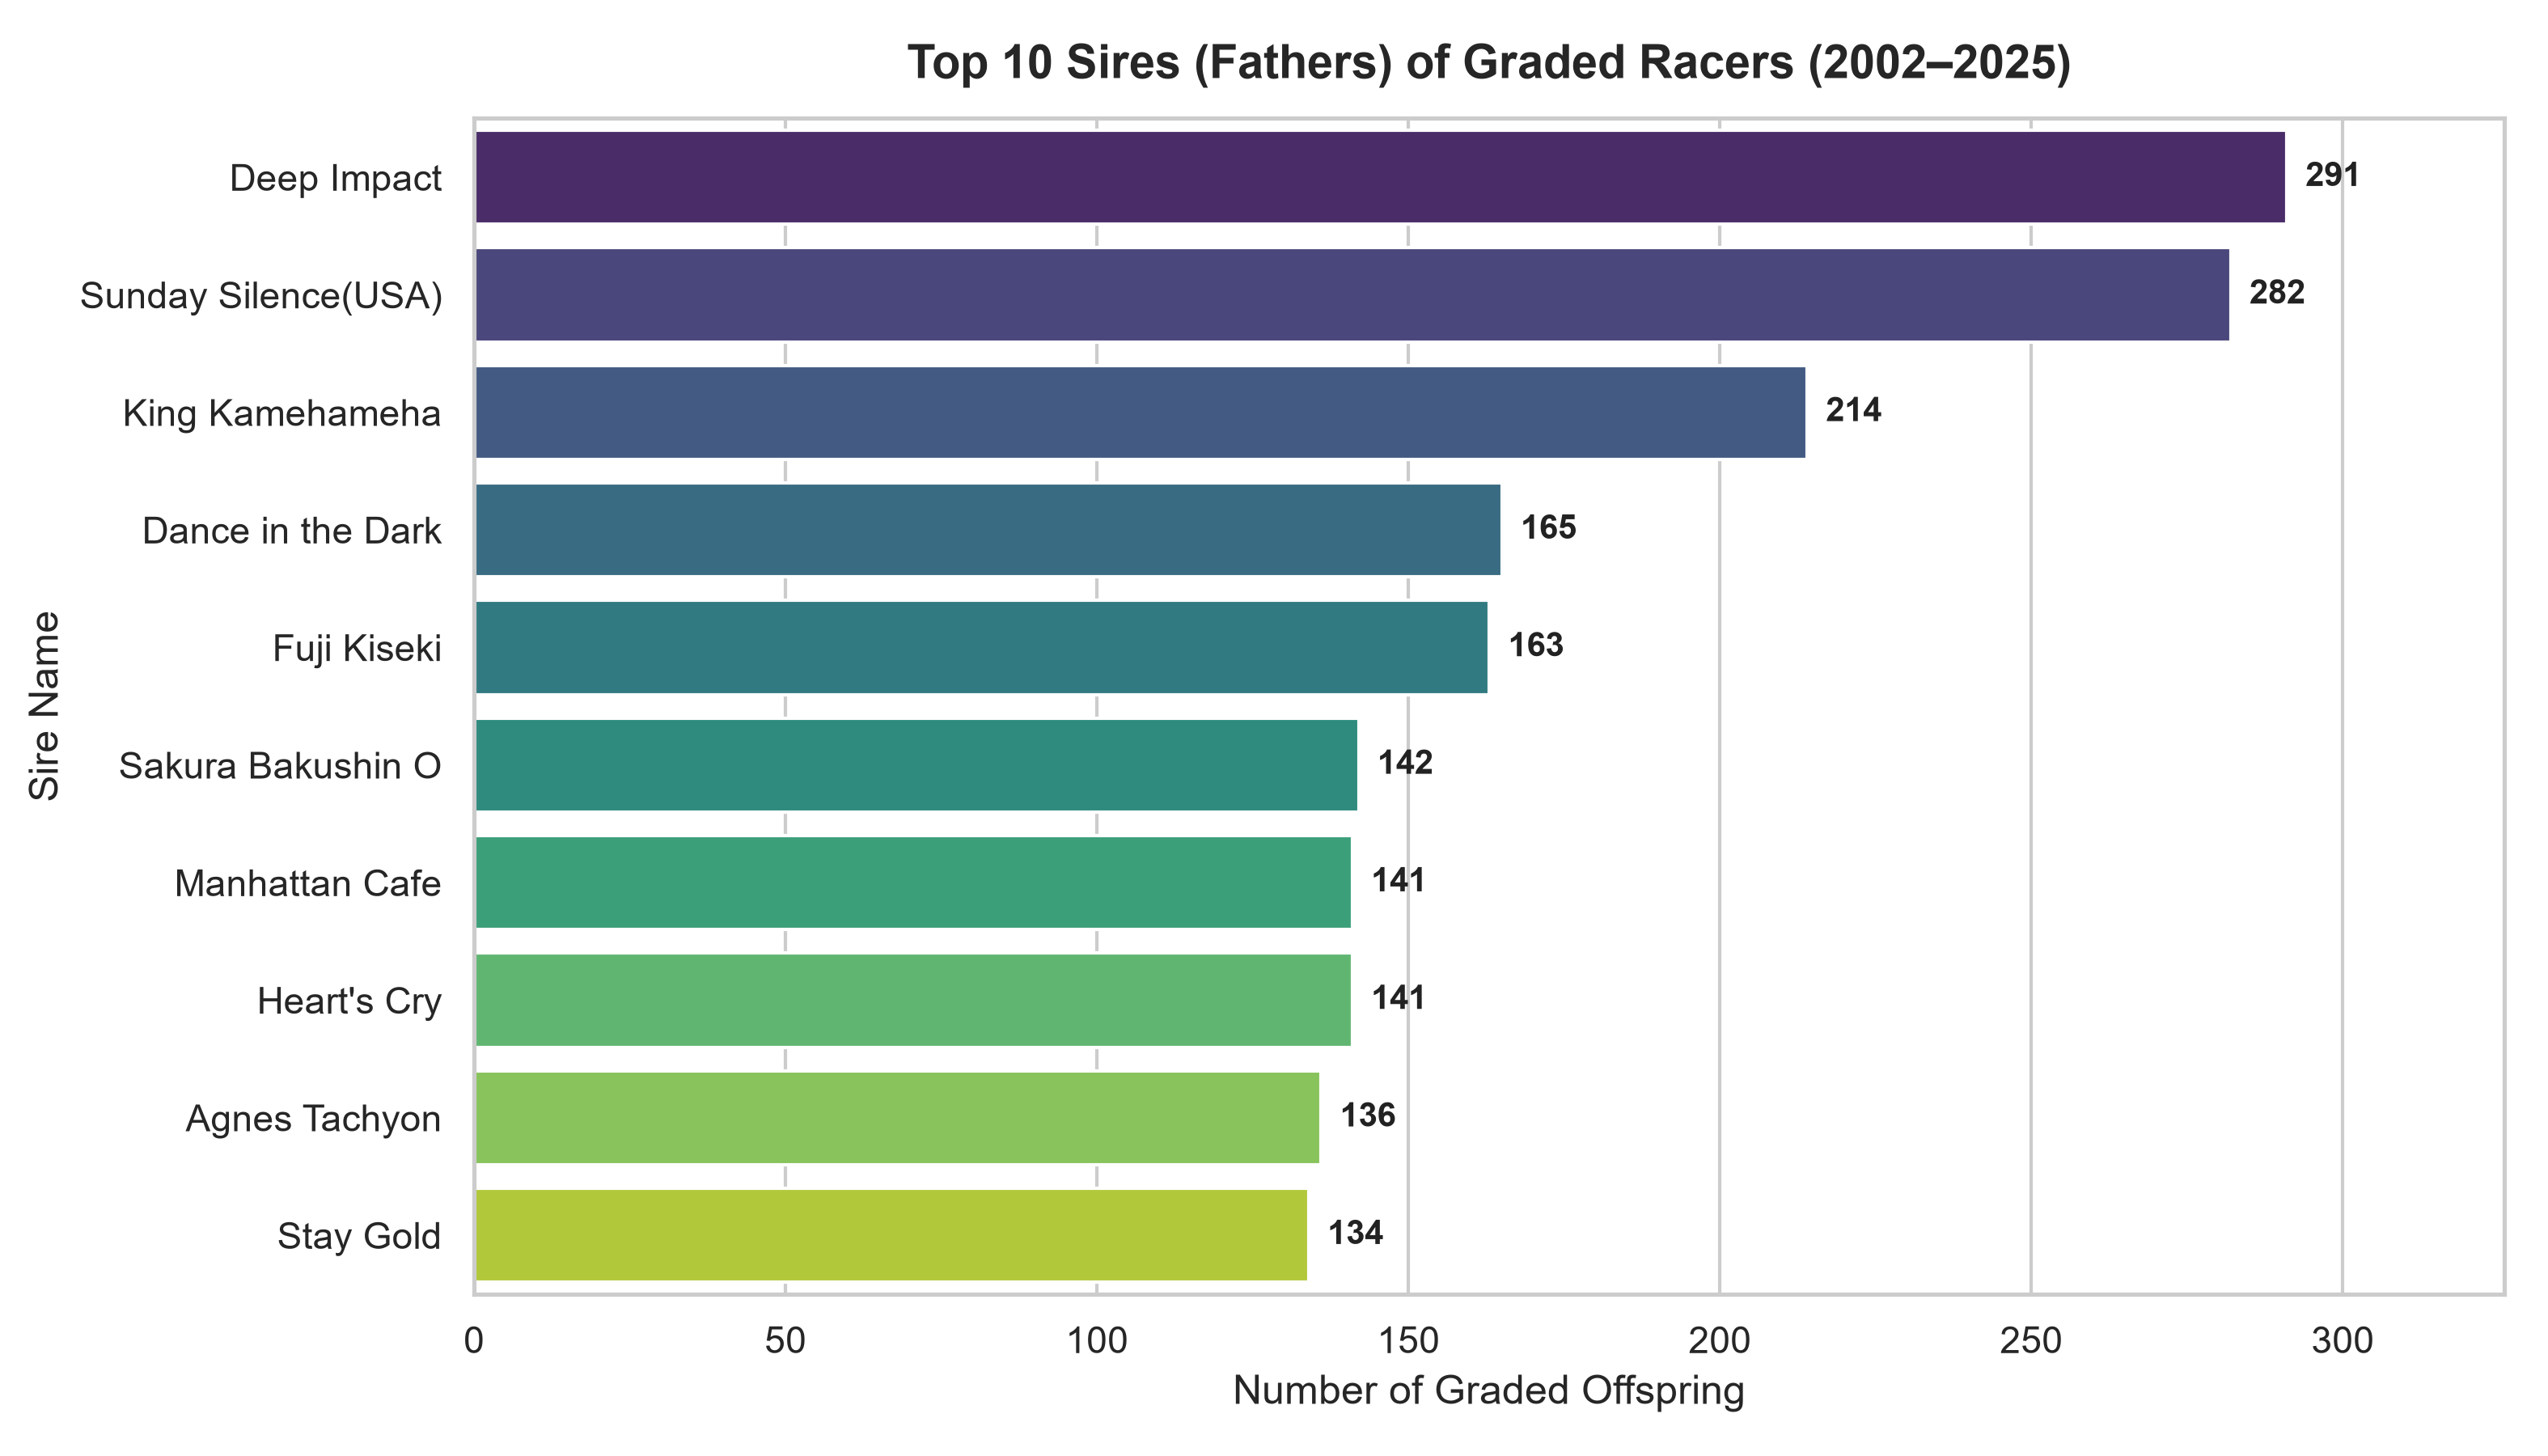
\includegraphics[width=0.98\textwidth]{../assets/top_sires.png}
\vspace{1mm}
{\scriptsize \textbf{Análise:} \textit{Deep Impact} (289 filhos Graded, 46 G1s) e seu pai \textit{Sunday Silence} (281 filhos, 42 G1s) lideram a era moderna.}
\end{column}
\begin{column}{0.50\textwidth}
\centering
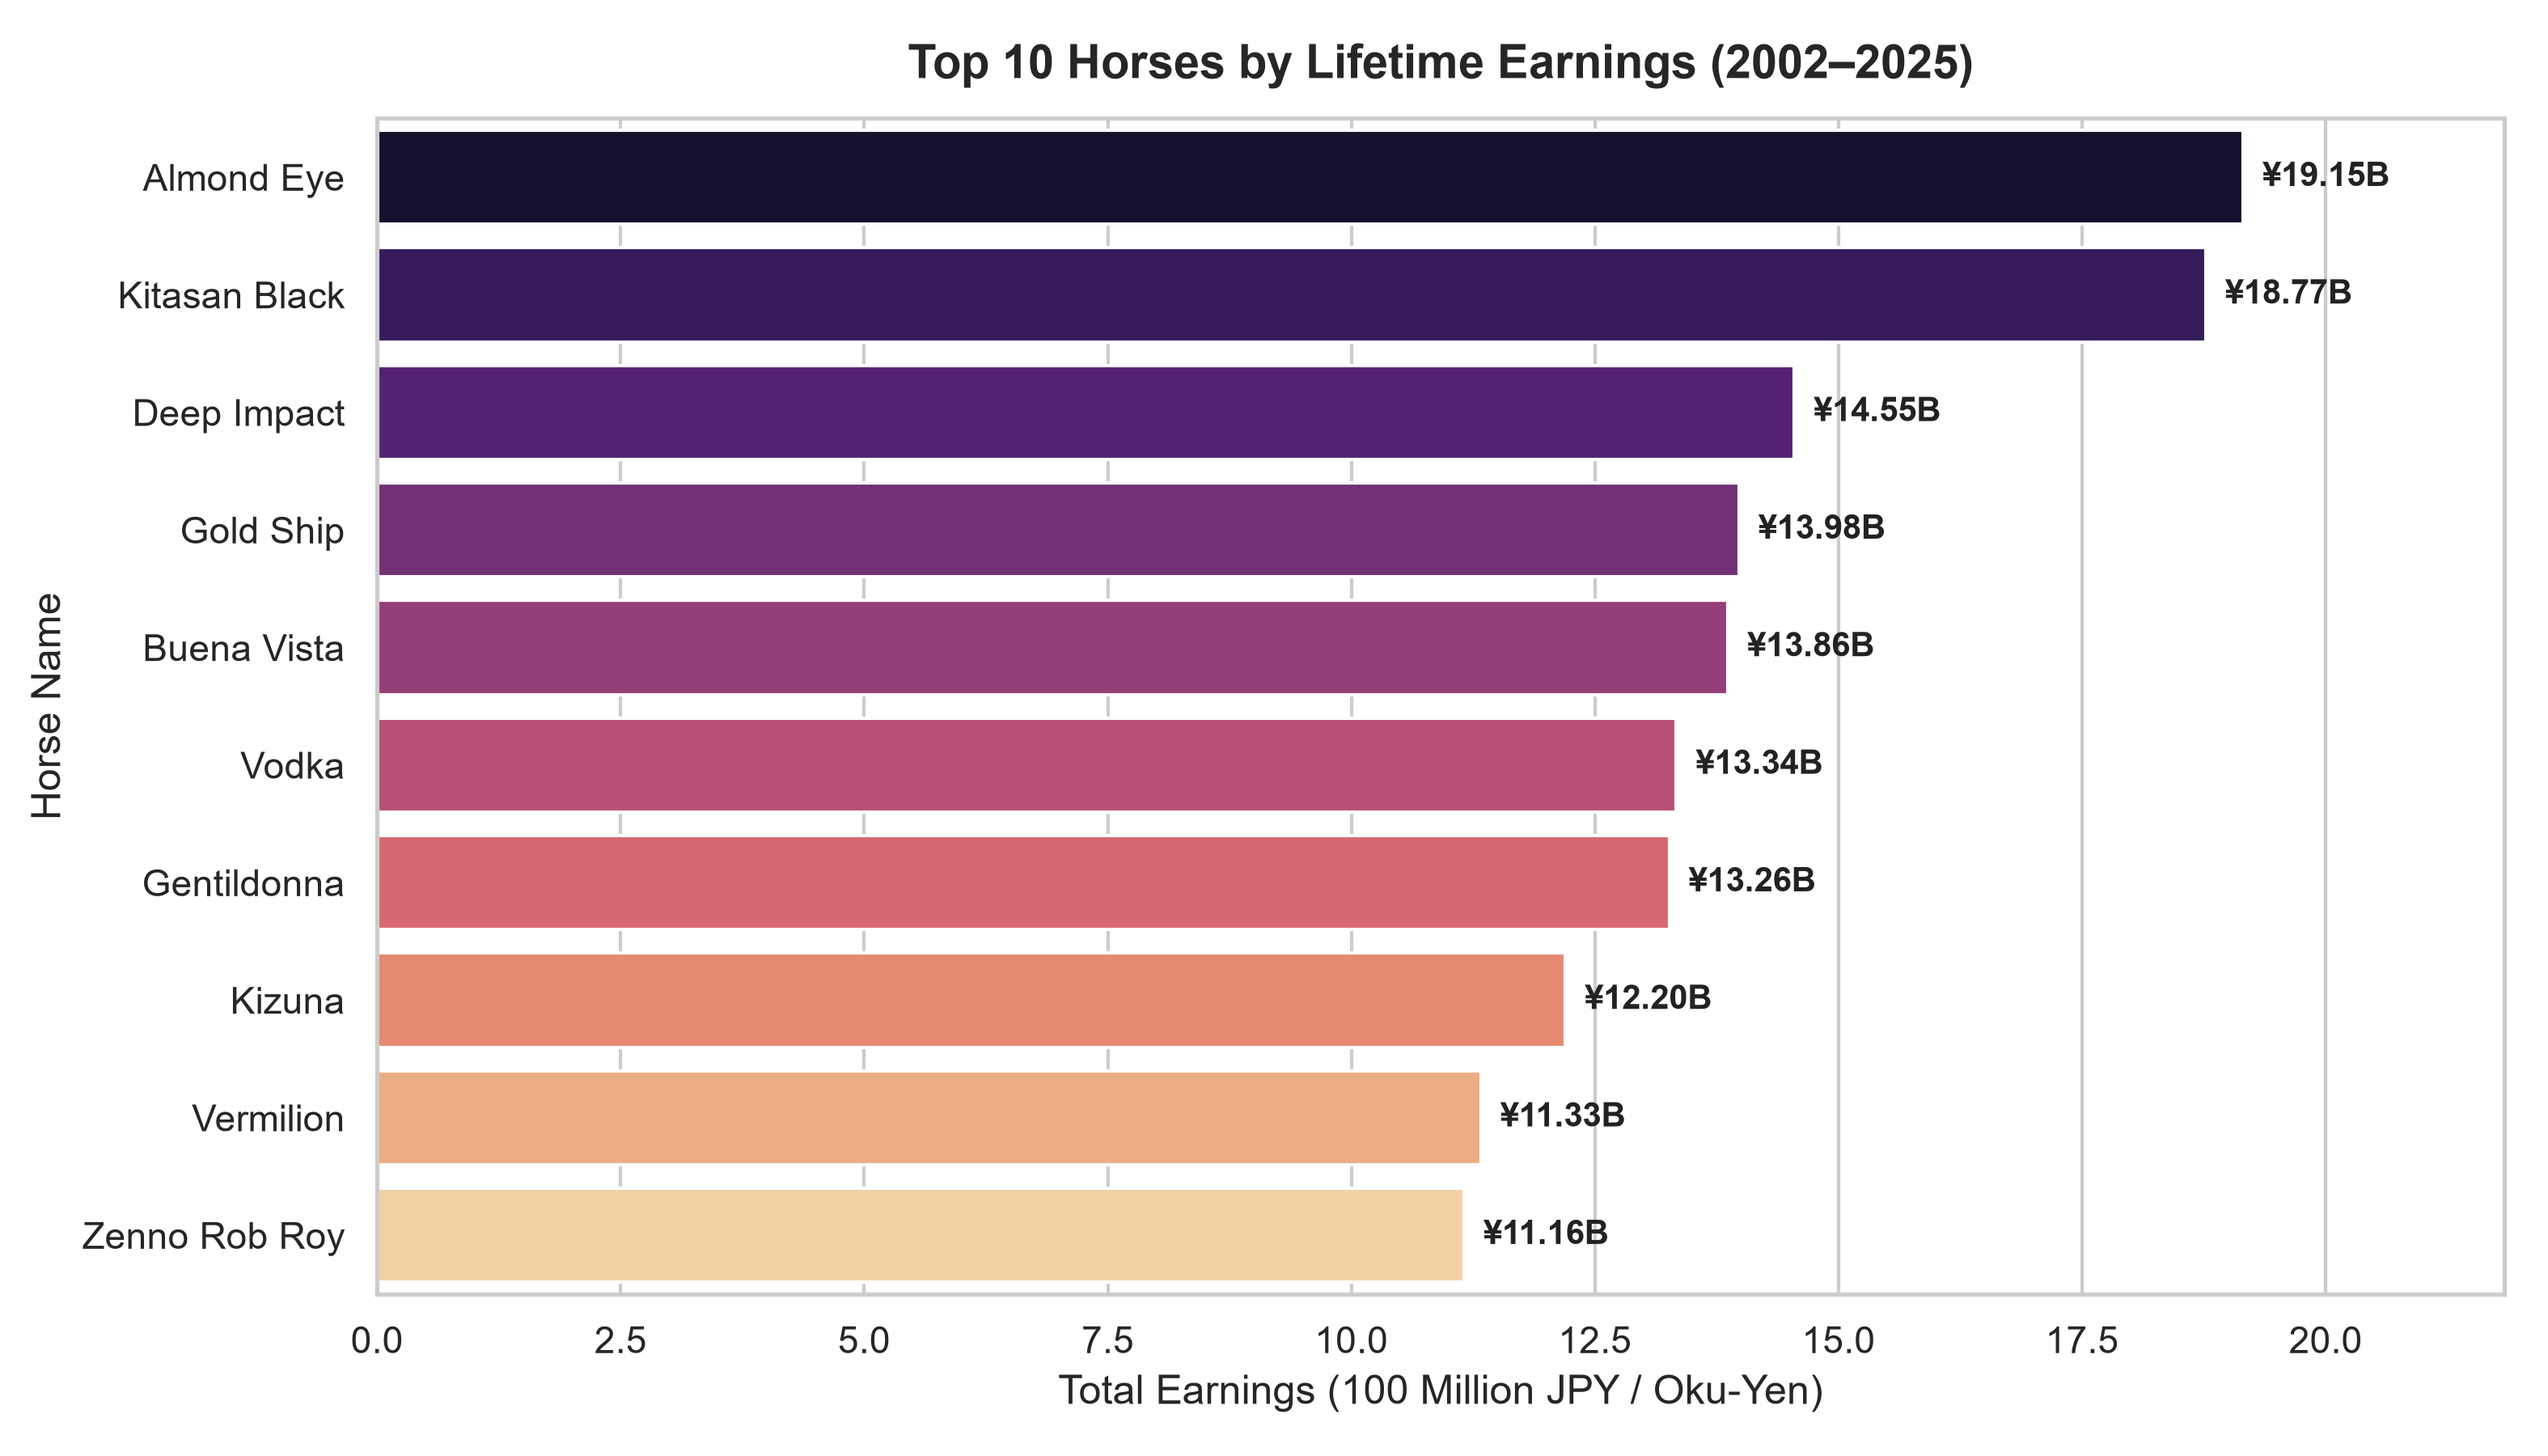
\includegraphics[width=0.98\textwidth]{../assets/top_earners.png}
\vspace{1mm}
{\scriptsize \textbf{Análise:} \textit{Almond Eye} (¥19,15B) e \textit{Kitasan Black} (¥18,77B) lideram os ganhos vitalícios em centenas de milhões de ienes.}
\end{column}
\end{columns}
\end{frame}

% SLIDE 6: VISUALIZAÇÃO 2 - DIAGRAMA SANKEY ALUVIAL (ESTILO SUPERSET)
\begin{frame}{5. Visualização Multidimensional: Diagrama Sankey Aluvial (4 Estágios)}
\centering
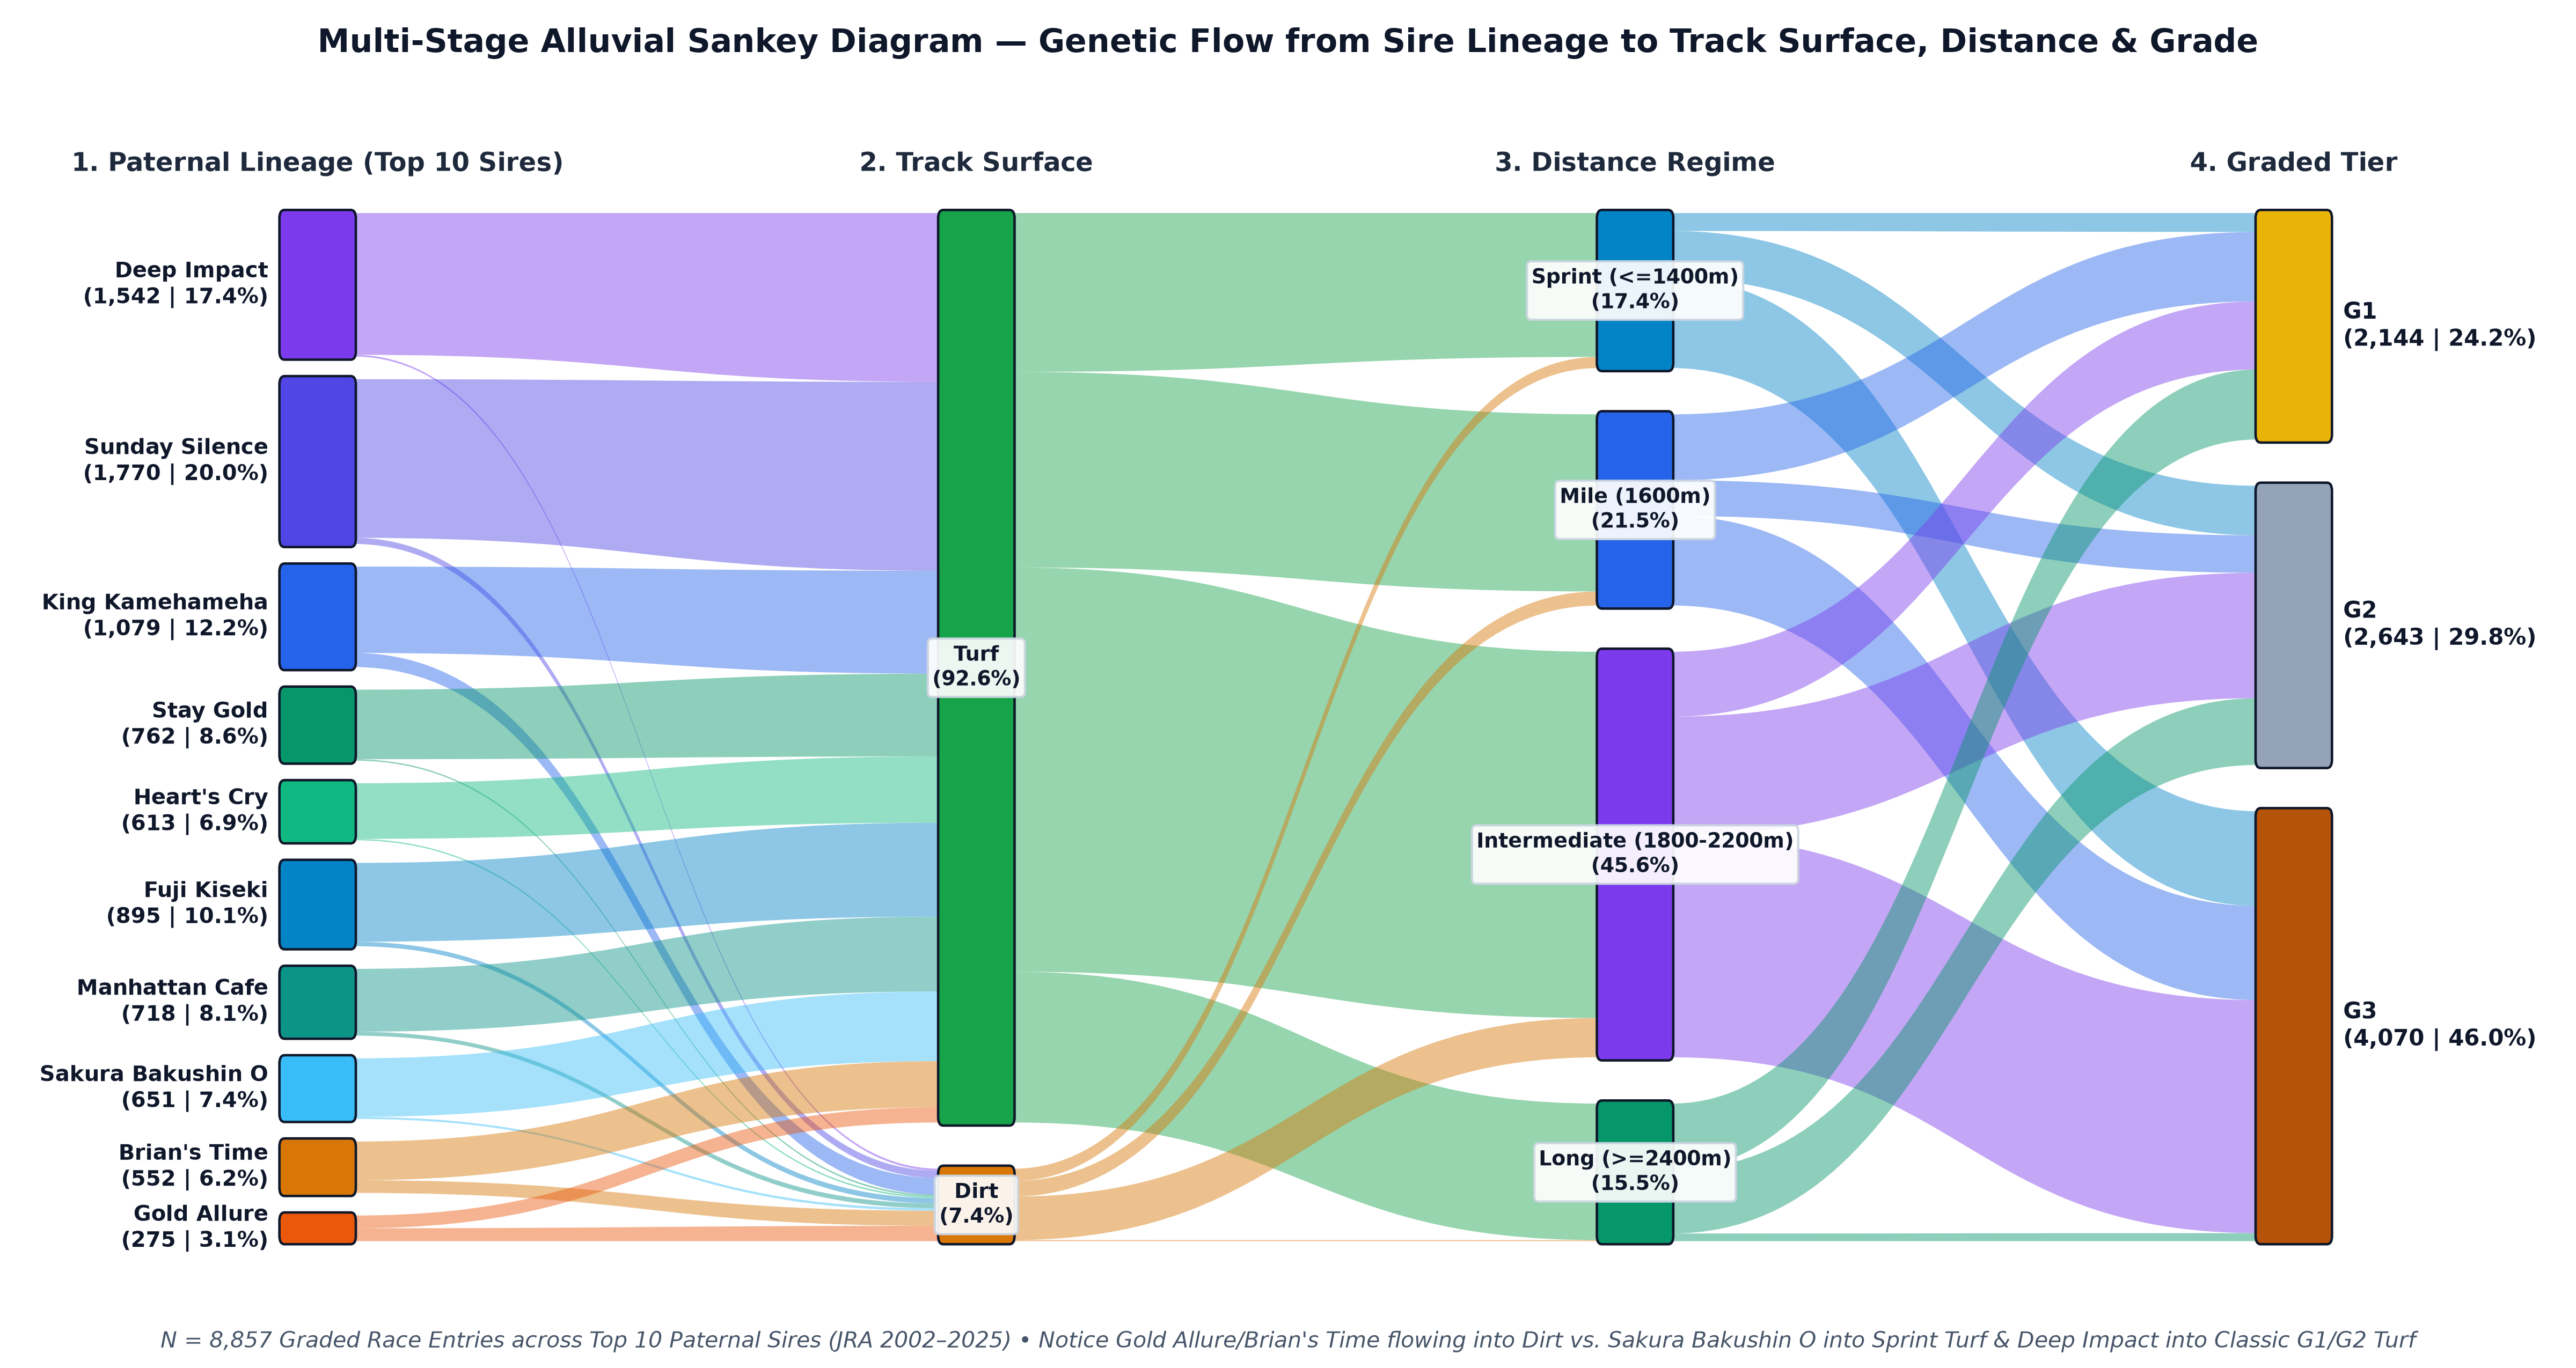
\includegraphics[width=0.88\textwidth]{../assets/superset_alluvial_sankey_flow.png}
\vspace{1mm}
\begin{itemize}
    \footnotesize
    \item \textbf{Codificação Multidimensional (\textit{DataViz Project / Apache Superset}):} Conecta simultaneamente \textit{Linhagem Paterna} $\to$ \textit{Superfície} $\to$ \textit{Regime de Distância} $\to$ \textit{Grau (G1/G2/G3)} ($N = 8.857$).
    \item \textbf{Achado Visual:} Fitas laranjas de \textit{Gold Allure} e \textit{Brian's Time} escoam para a \textbf{Areia (\textit{Dirt})}; \textit{Sakura Bakushin O} flui para \textbf{Sprint ($\le 1400\text{m}$)}; e \textit{Deep Impact} domina as distâncias clássicas de Grama rumo ao \textbf{G1}.
\end{itemize}
\end{frame}

% SLIDE 7: VISUALIZAÇÃO 3 - RADAR (DIAMANTE INJUSTIÇADO) E SUNBURST
\begin{frame}{6. PageRank ($H_2$): ``Diamantes Injustiçados'' (Radar) \& Sunburst}
\centering
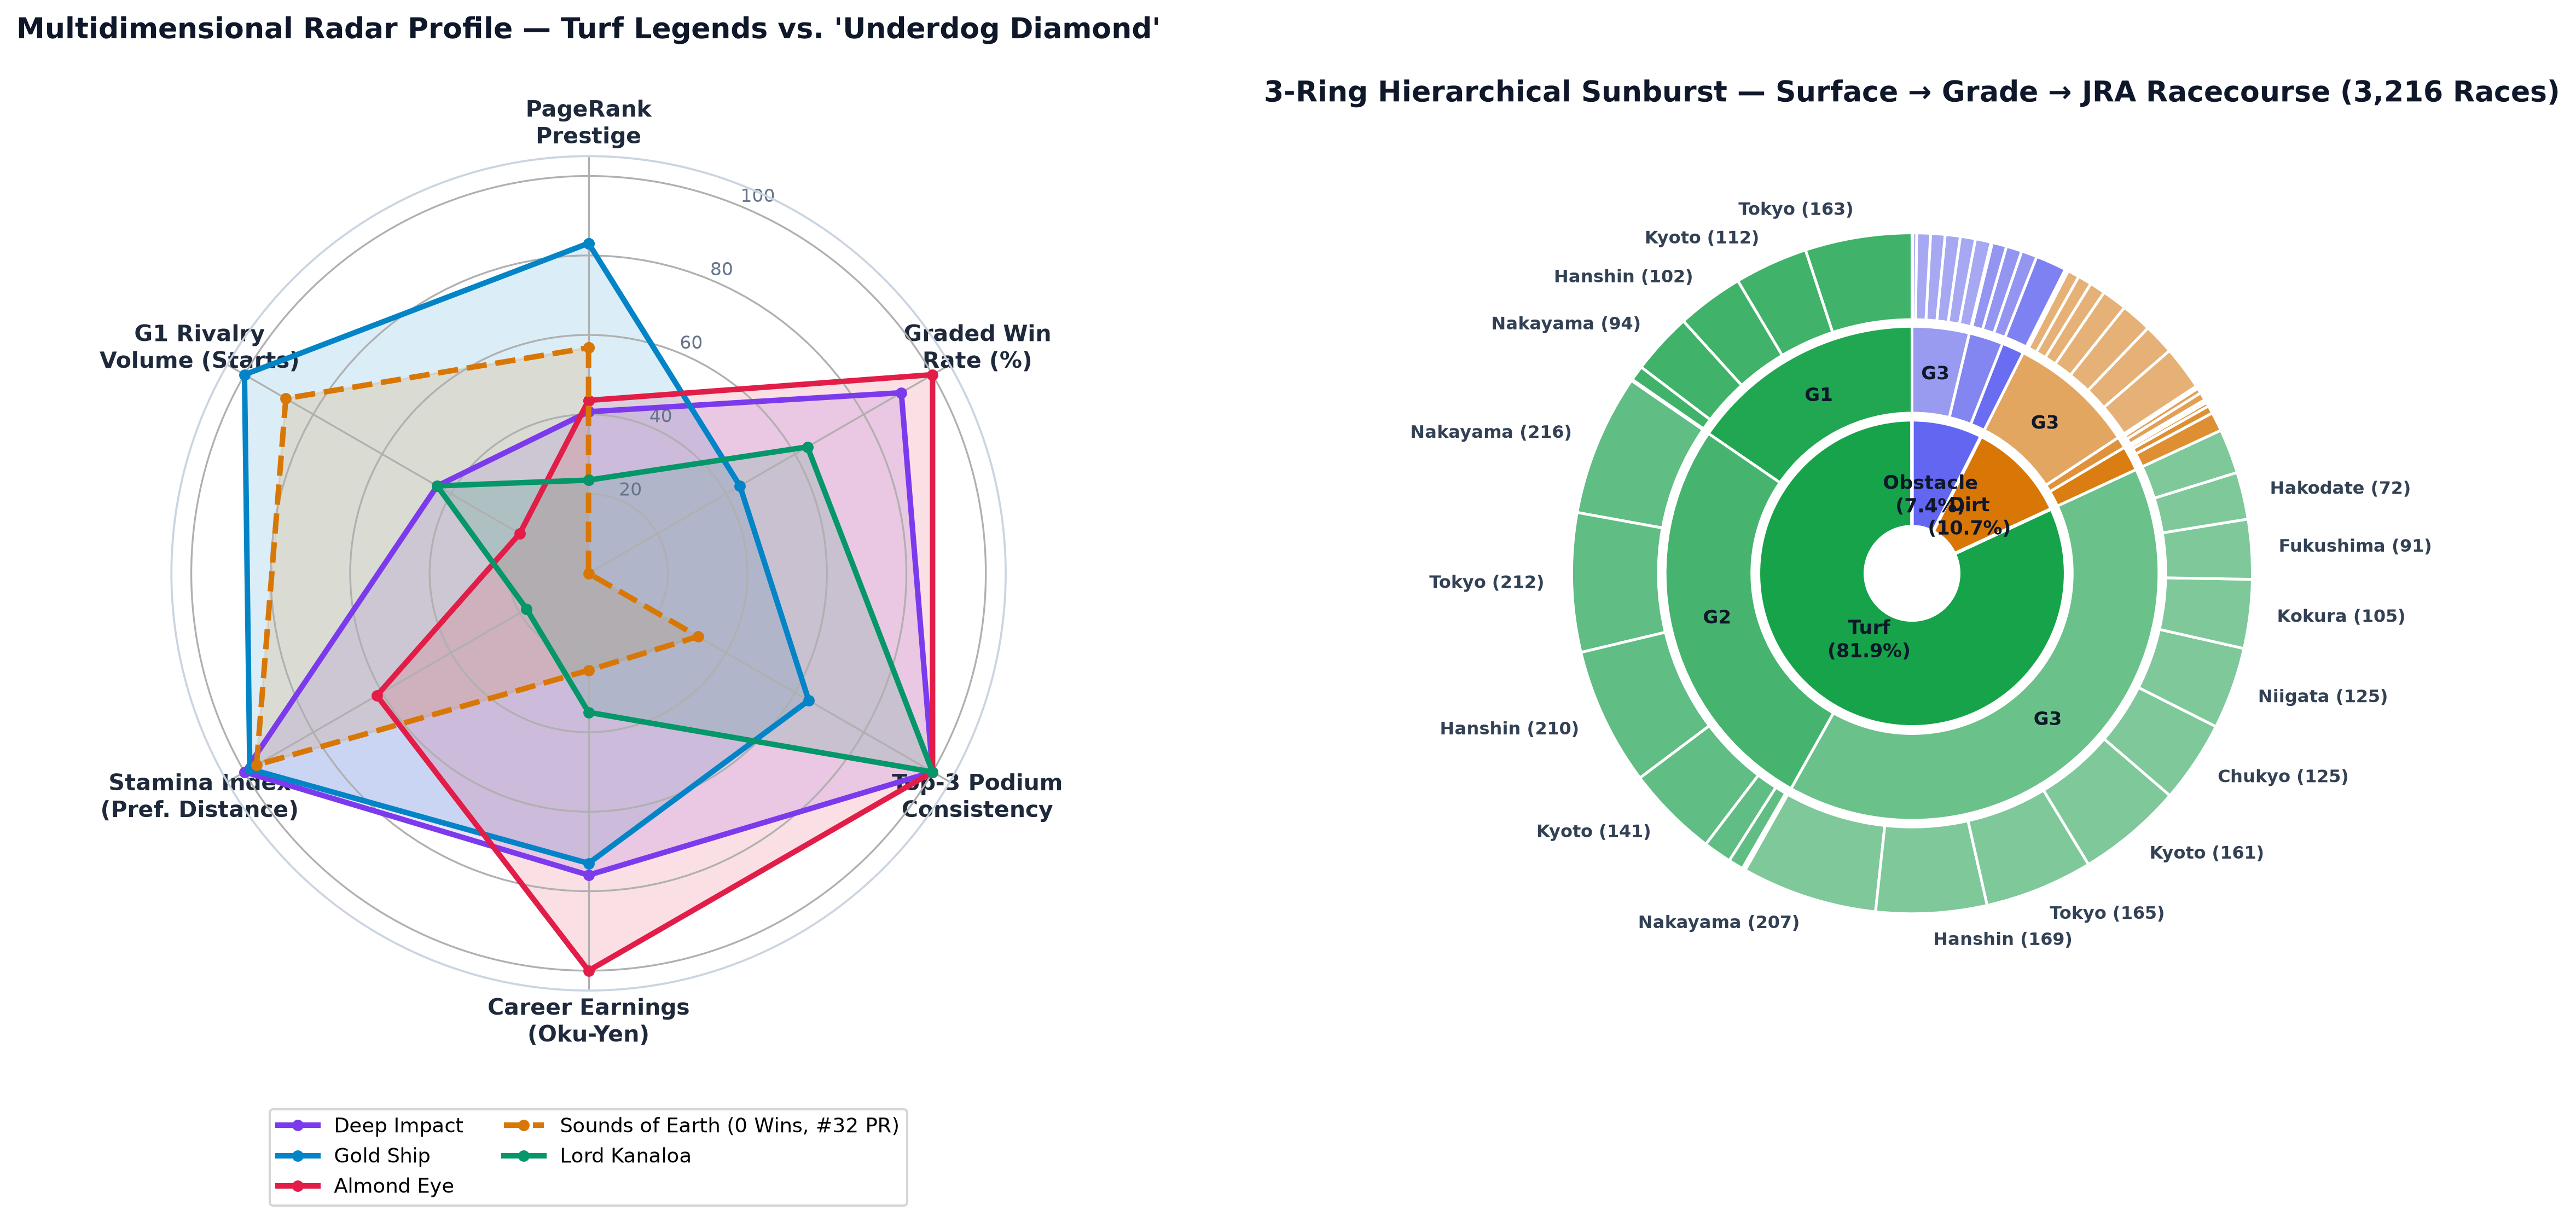
\includegraphics[width=0.88\textwidth]{../assets/superset_radar_and_sunburst.png}
\vspace{1mm}
\begin{itemize}
    \footnotesize
    \item \textbf{A Descoberta dos ``Diamantes Injustiçados'' ($r = 0,8799$ com pódios):} O cavalo \textbf{\textit{Sounds of Earth}} tem \textbf{0 vitórias Graded}, mas ocupa a \textbf{32ª posição geral entre 8.135 cavalos} no PageRank graças a 7 pódios de elite (vices no Japan Cup G1, Arima Kinen G1 e Kikuka Sho G1)! Veja no Radar o vértice de vitórias em $0\%$ e o PageRank/Volume G1 no topo!
    \item \textbf{Sunburst Hierárquico (3.216 corridas):} Mapeia \textit{Superfície} (81,9\% Grama, 10,7\% Areia, 7,4\% Obstáculos) $\to$ \textit{Grau} $\to$ \textit{10 Hipódromos}.
\end{itemize}
\end{frame}

% SLIDE 8: VISUALIZAÇÃO 4 - STREAMGRAPH DE DINASTIAS
\begin{frame}{7. Evolução Temporal: Streamgraph das 12 Grandes Dinastias}
\centering
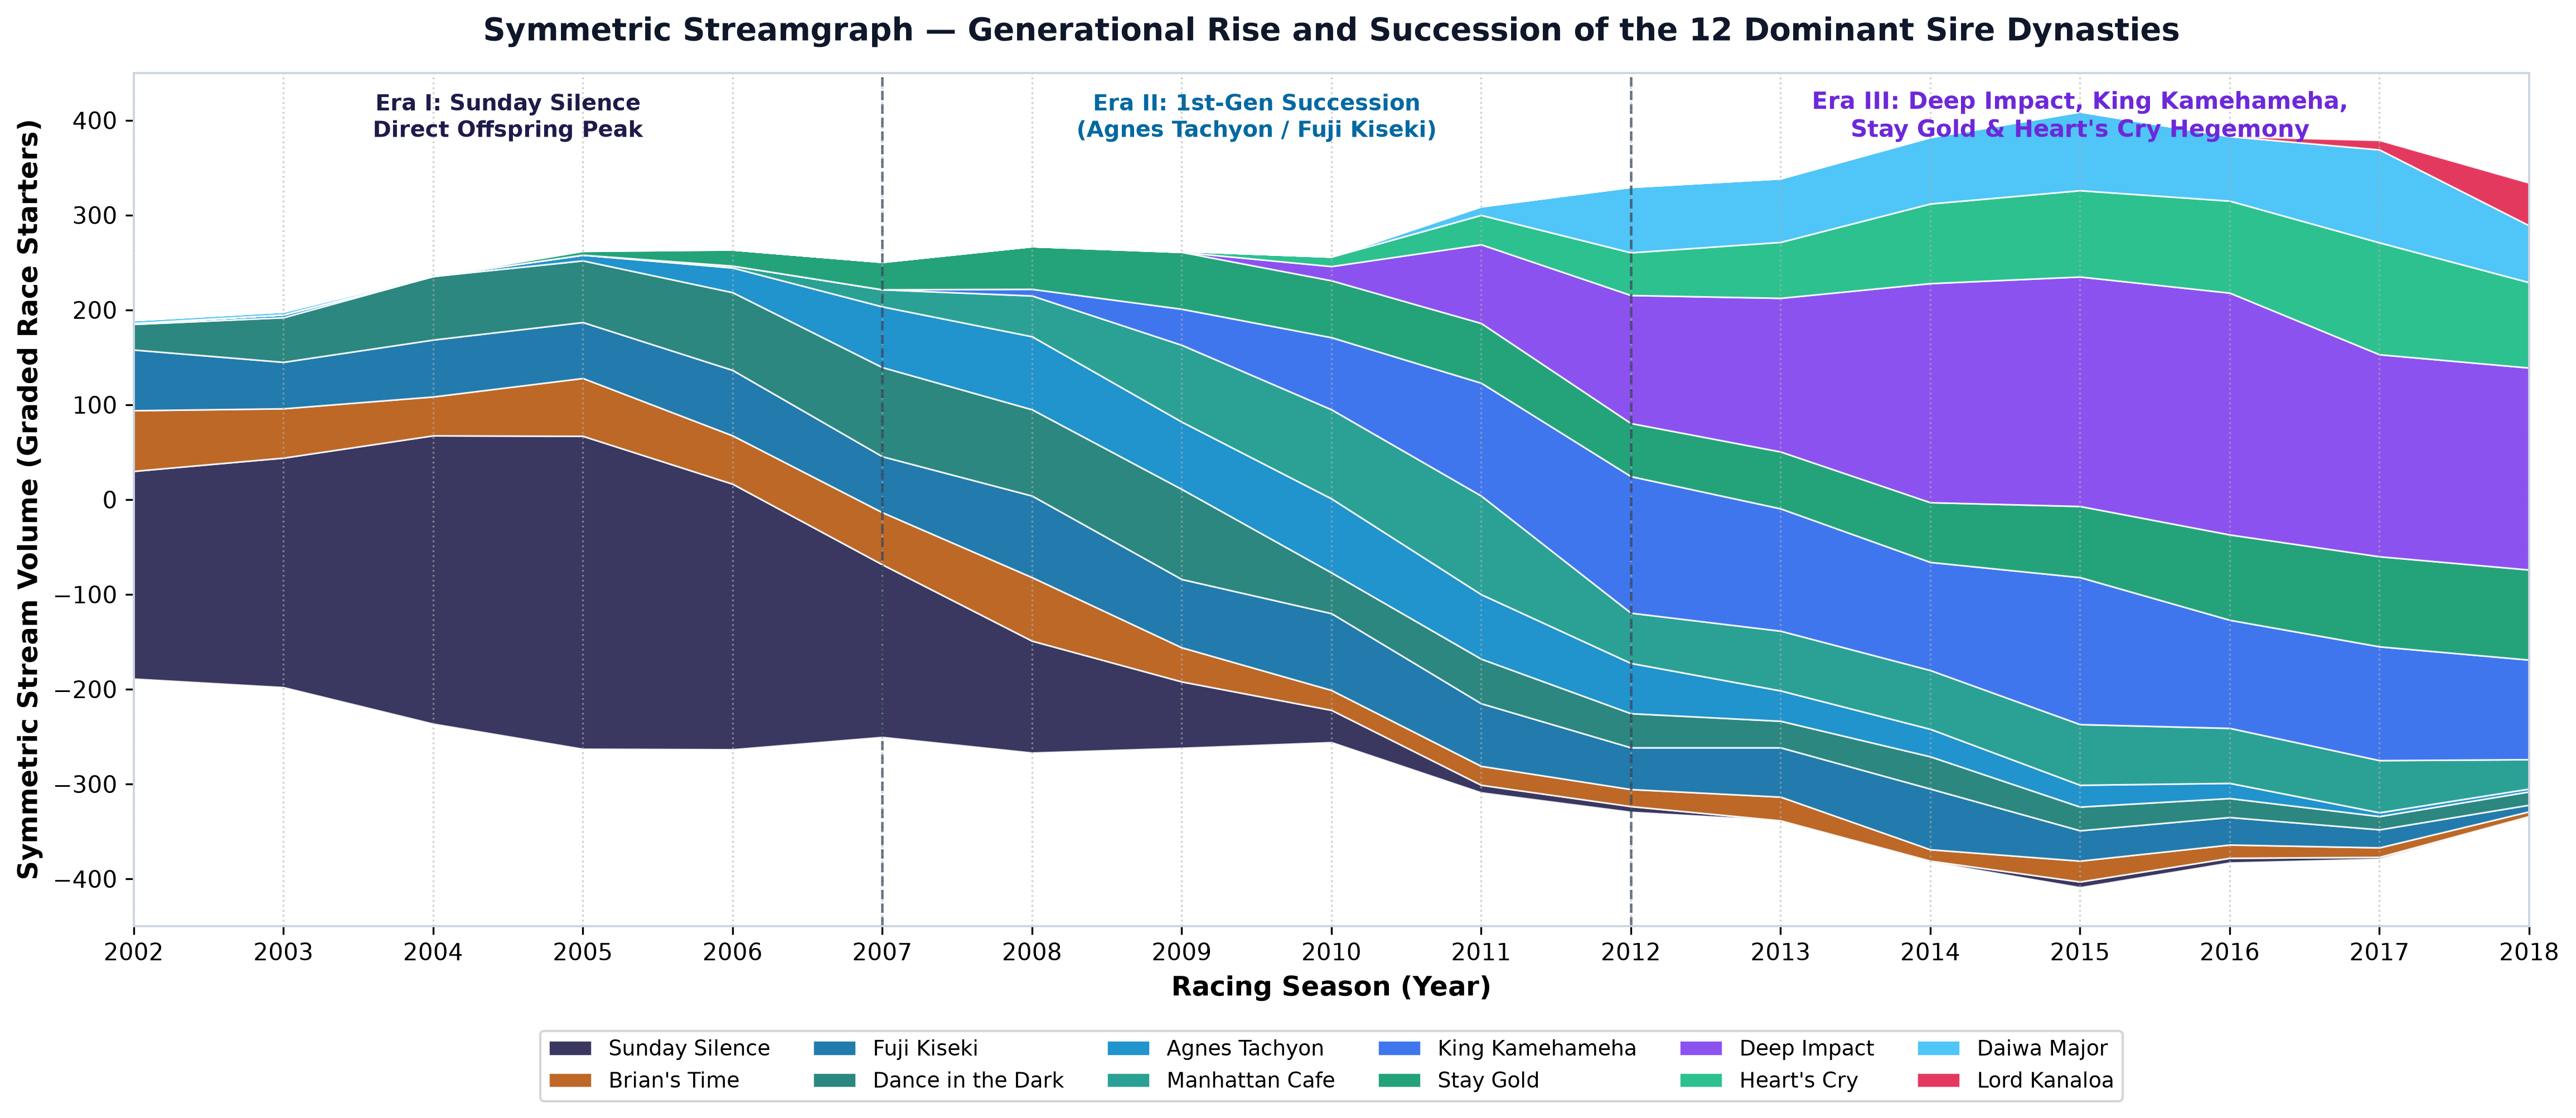
\includegraphics[width=0.88\textwidth]{../assets/superset_streamgraph_dynasties.png}
\vspace{1mm}
\begin{itemize}
    \footnotesize
    \item \textbf{Transição Geracional em 3 Eras:}
    \item \textbf{Era I (2002--2007):} Hegemonia dos filhos diretos de \textit{Sunday Silence} e \textit{Brian's Time}.
    \item \textbf{Era II (2008--2012):} Sucessão pela 1ª geração nacional (\textit{Agnes Tachyon}, \textit{Fuji Kiseki}, \textit{Dance in the Dark}, \textit{Manhattan Cafe}).
    \item \textbf{Era III (2013+):} Domínio de \textit{Deep Impact}, \textit{King Kamehameha}, \textit{Stay Gold}, \textit{Heart's Cry} e ascensão de \textit{Lord Kanaloa}.
\end{itemize}
\end{frame}

% SLIDE 9: VISUALIZAÇÃO 5 - SPLIT-VIOLIN BIOMÉTRICO E COORDENADAS PARALELAS
\begin{frame}{8. Biometria Equina (Split-Violin) \& Coordenadas Paralelas}
\centering
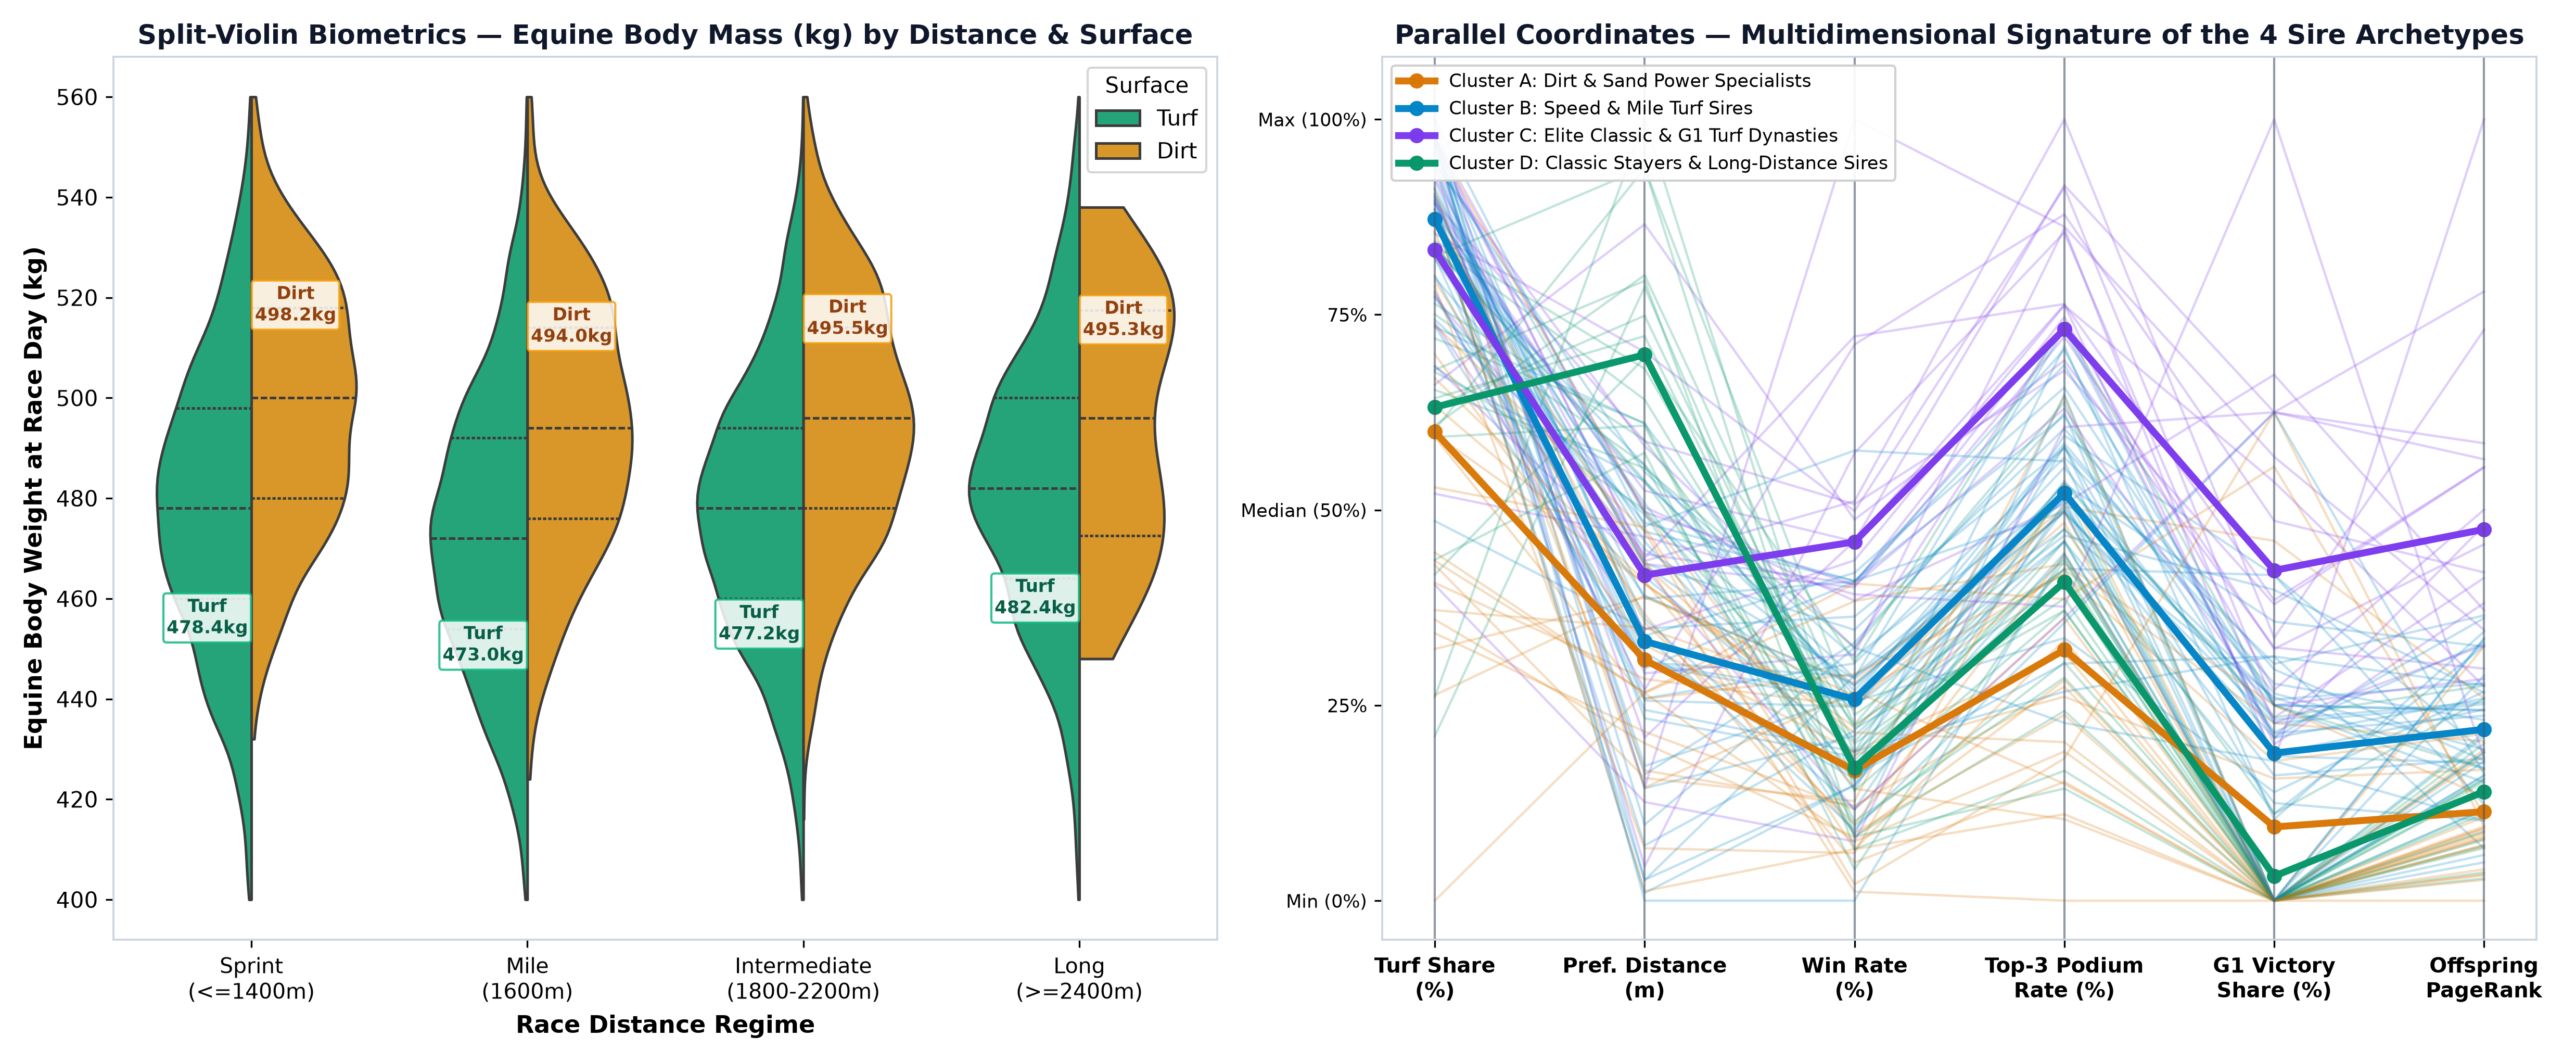
\includegraphics[width=0.88\textwidth]{../assets/superset_raincloud_and_parallel.png}
\vspace{1mm}
\begin{itemize}
    \footnotesize
    \item \textbf{Descoberta Biométrica (Esquerda):} Em todos os regimes de distância, competidores de \textbf{Areia (\textit{Dirt}, $\approx 494\text{--}498\text{ kg}$)} são \textbf{16 kg a 21 kg mais pesados e musculosos} que os de \textbf{Grama (\textit{Turf}, $\approx 473\text{--}482\text{ kg}$)}.
    \item \textbf{Coordenadas Paralelas (Direita):} Traça a assinatura multidimensional dos 106 garanhões nos 6 indicadores zootécnicos.
\end{itemize}
\end{frame}

% SLIDE 10: MACHINE LEARNING 1 - K-MEANS++ PCA 2D
\begin{frame}{9. Aprendizado Não-Supervisionado: K-Means++ \& PCA 2D}
\centering
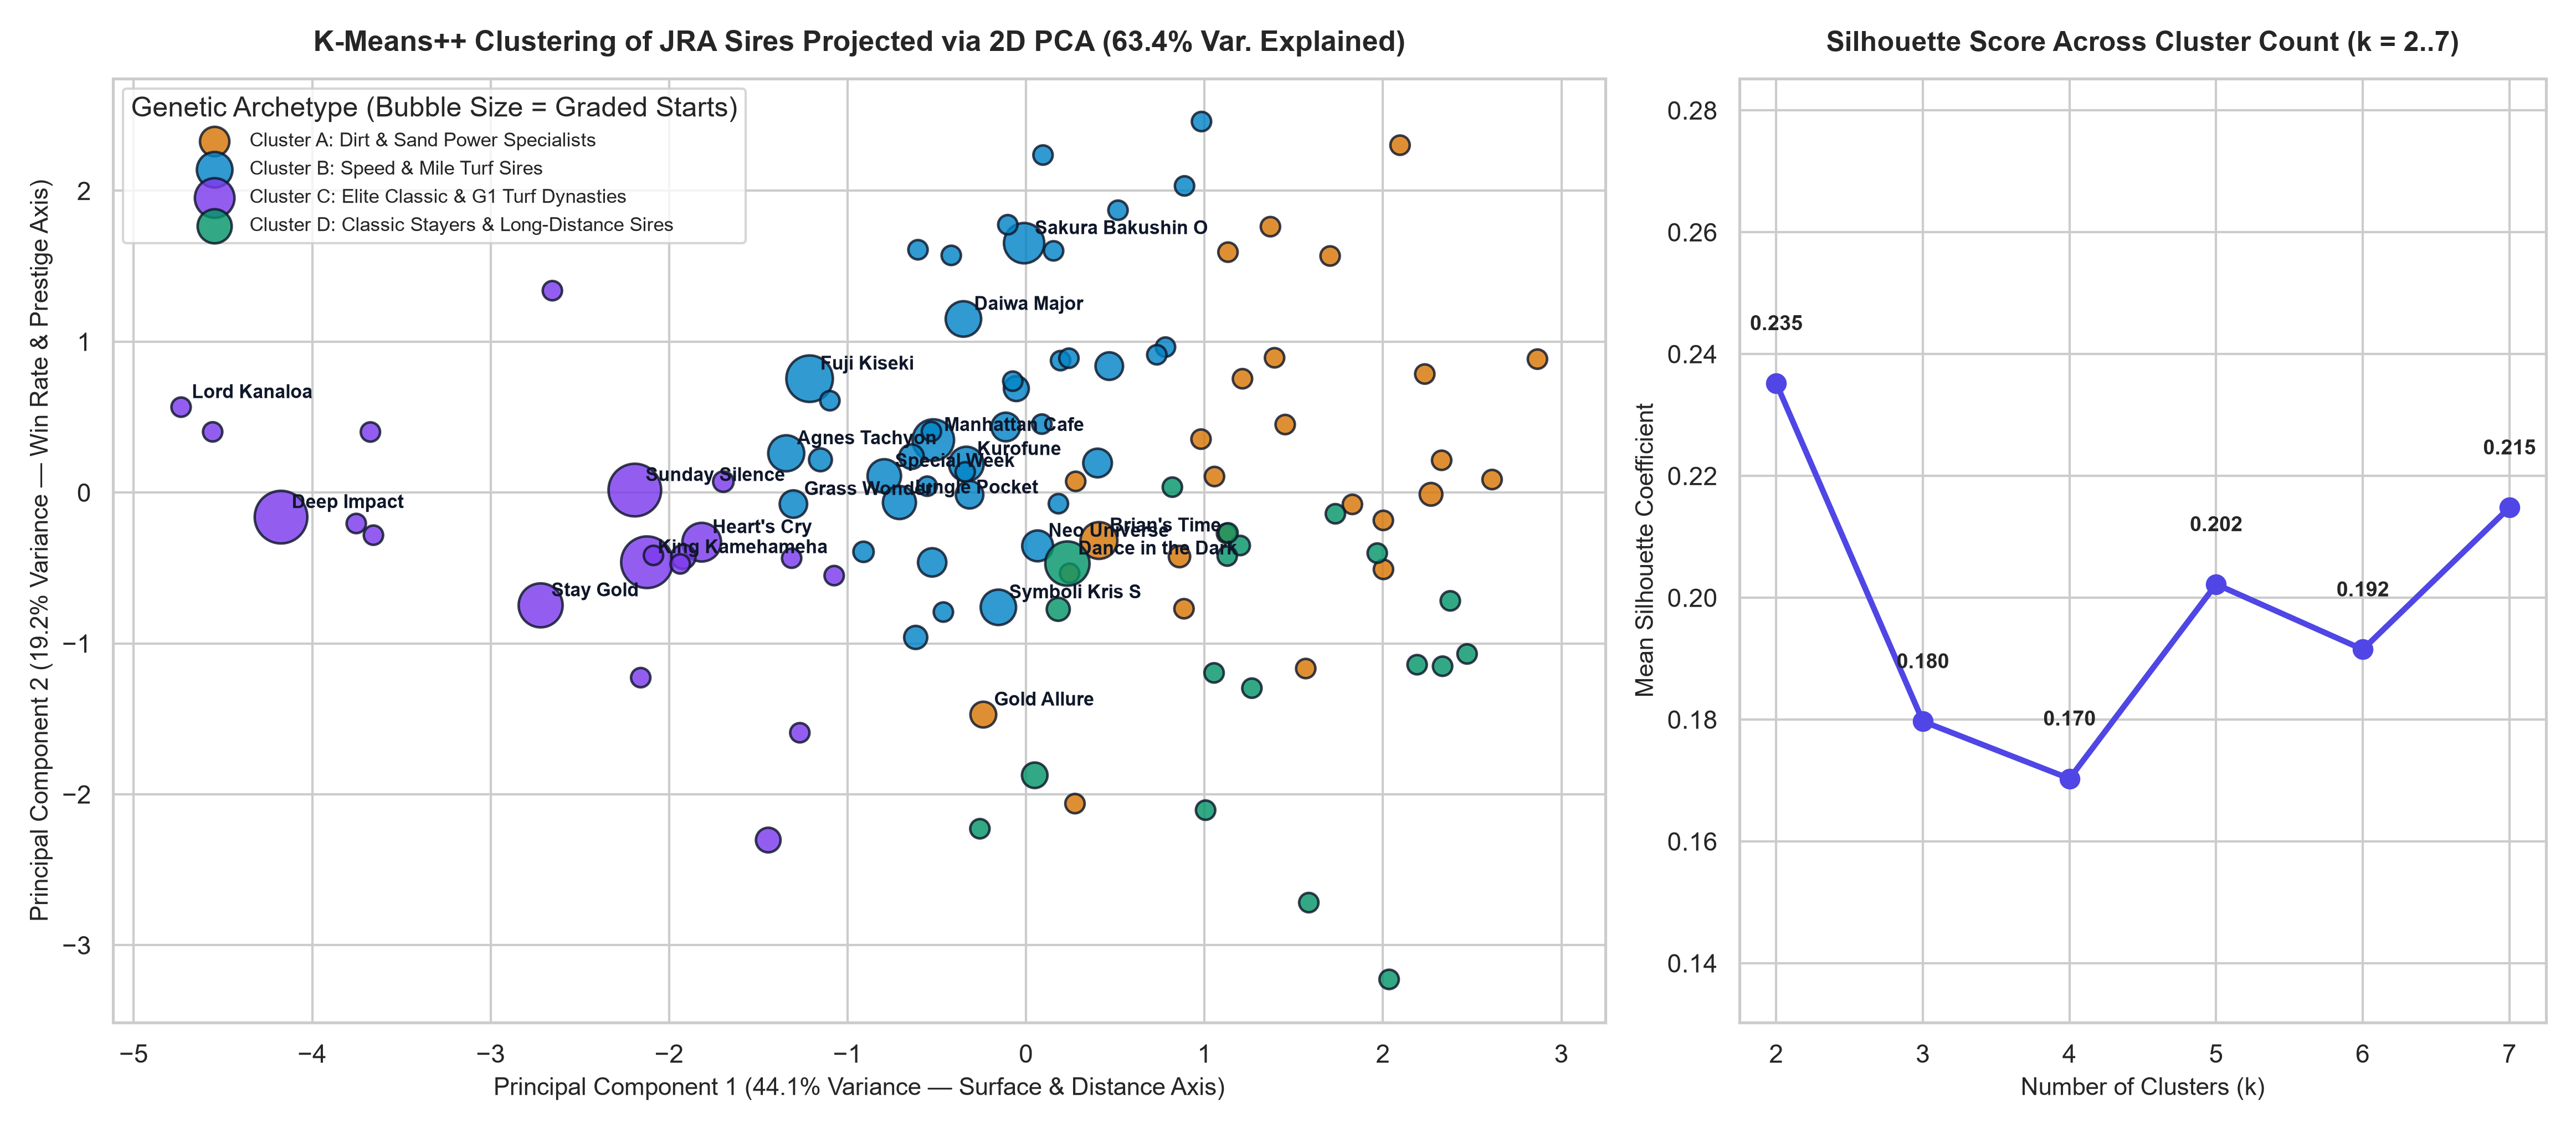
\includegraphics[width=0.86\textwidth]{../assets/ml_kmeans_pca_clusters.png}
\vspace{1mm}
\begin{itemize}
    \footnotesize
    \item \textbf{63,4\% da Variância Total Explicada em 2 Eixos ($\text{PC}_1 = 44,1\%$, $\text{PC}_2 = 19,2\%$):}
    \item \textbf{Cluster A (Laranja, $n=26$):} Especialistas de Areia (\textit{Gold Allure}, \textit{Brian's Time}).
    \item \textbf{Cluster B (Azul, $n=41$):} Velocistas e Milheiros de Grama (\textit{Sakura Bakushin O}, \textit{Fuji Kiseki}, \textit{Daiwa Major}).
    \item \textbf{Cluster C (Roxo, $n=20$):} Dinastias Clássicas de G1 (\textit{Deep Impact}, \textit{Sunday Silence}, \textit{King Kamehameha}, \textit{Stay Gold}).
    \item \textbf{Cluster D (Verde, $n=19$):} Fundistas / Stayers Clássicos (\textit{Dance in the Dark}, \textit{Mayano Top Gun}).
\end{itemize}
\end{frame}

% SLIDE 11: MACHINE LEARNING 2 - RANDOM FOREST E TESTE QUI-QUADRADO
\begin{frame}{10. Machine Learning Supervisionado (Random Forest) \& Testes $H_1$}
\centering
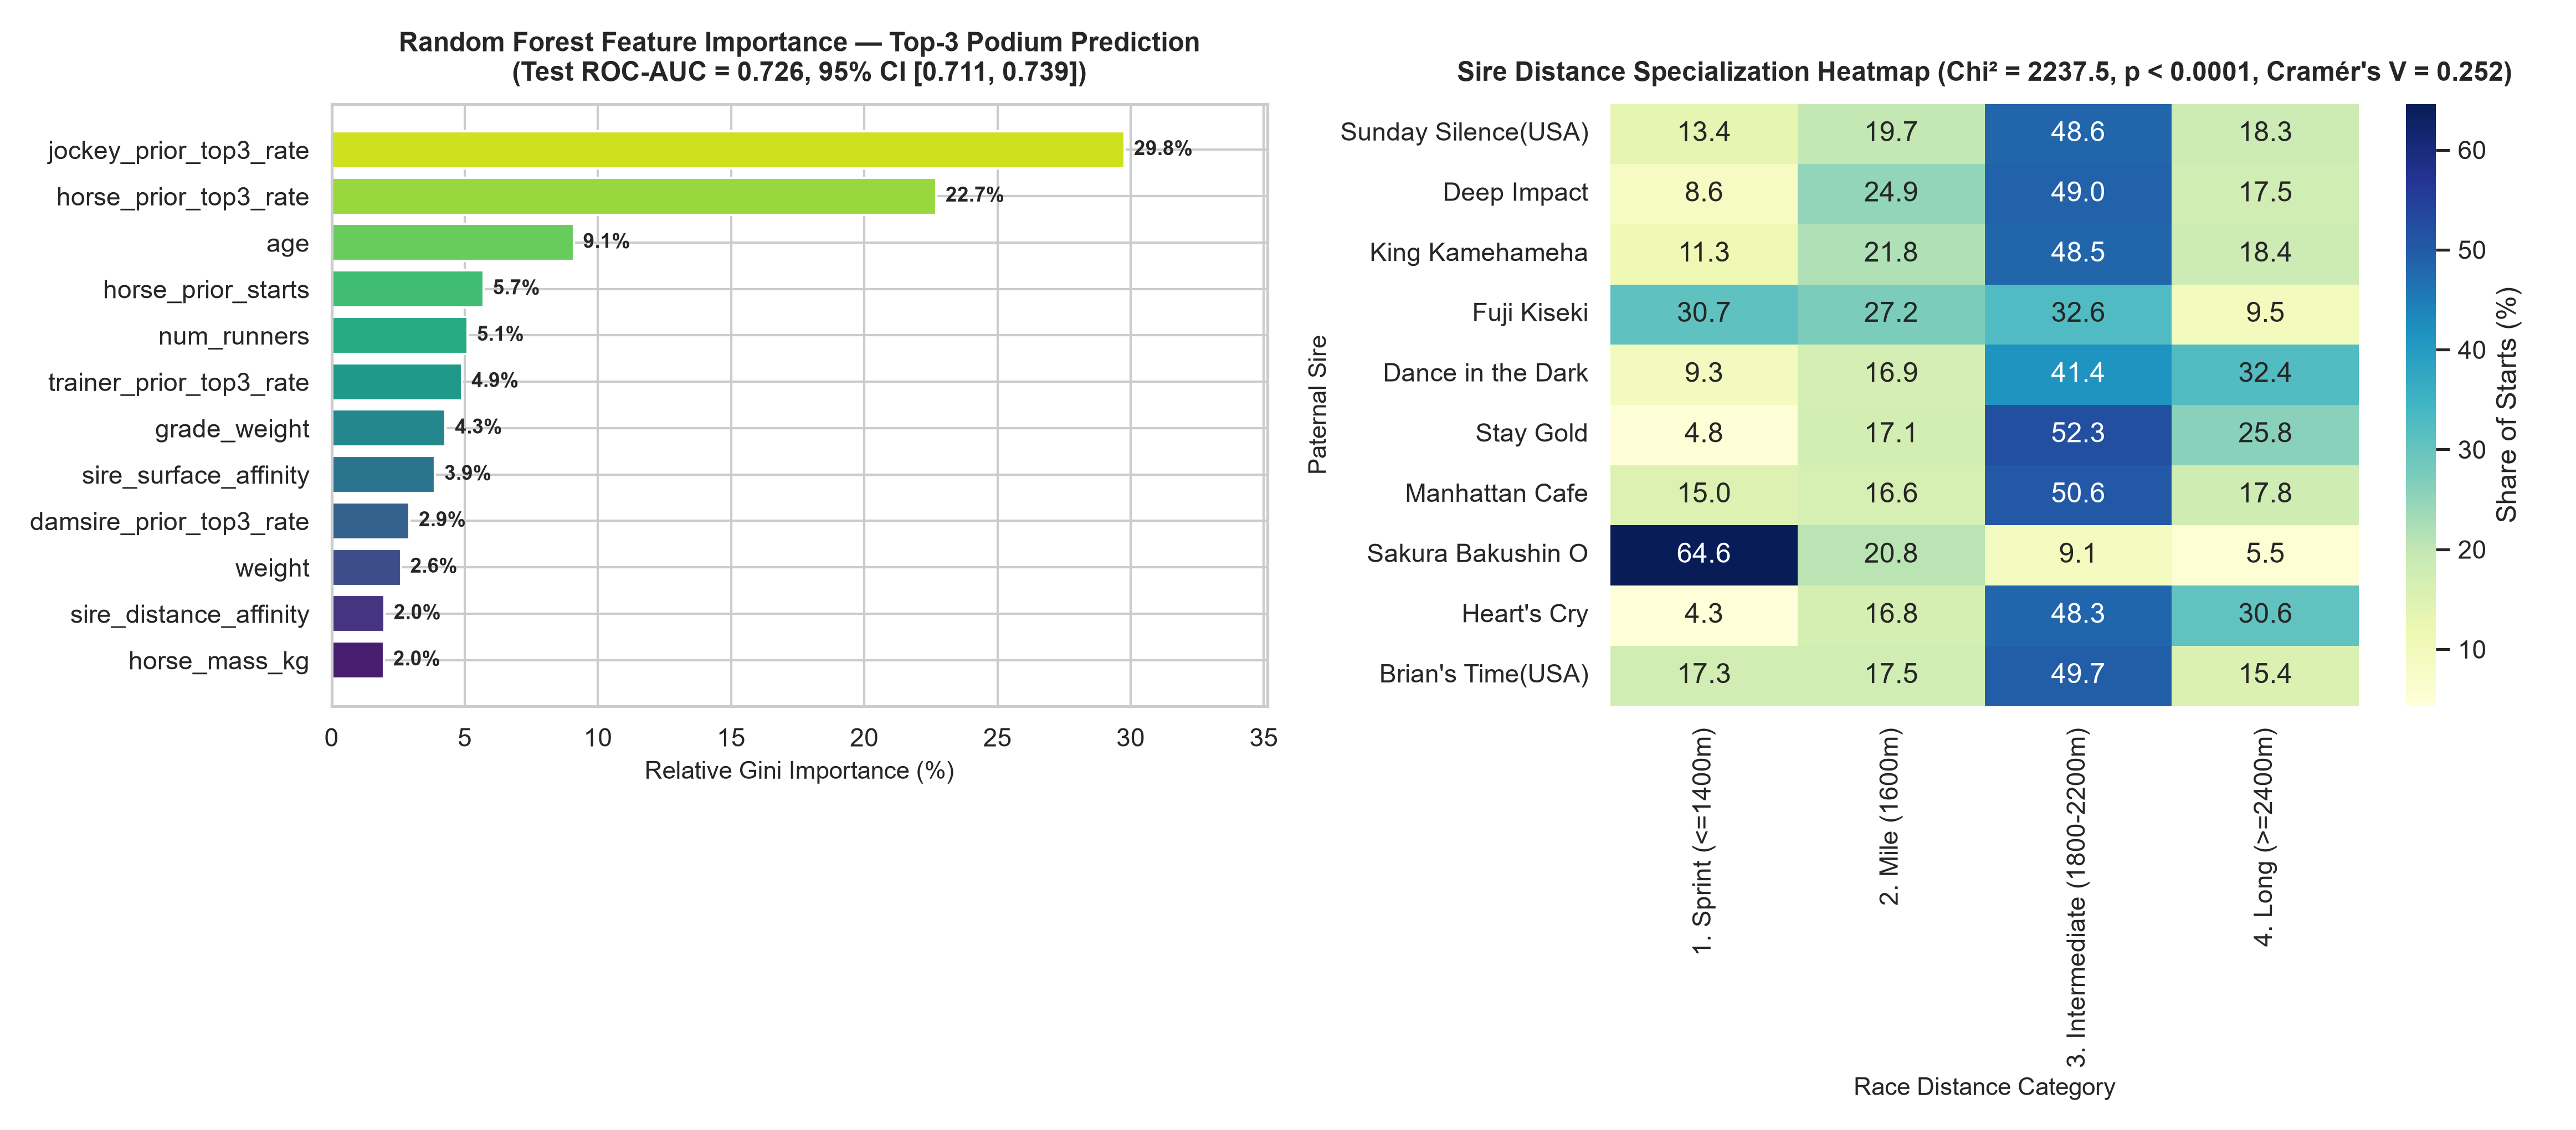
\includegraphics[width=0.85\textwidth]{../assets/ml_random_forest_and_chi2.png}
\vspace{1mm}
\begin{columns}[T]
\begin{column}{0.52\textwidth}
\footnotesize
\textbf{Predição Cronológica Out-of-Time (Teste 2016--2018, $N=5.889$, \textit{Zero Data Leakage}):}
\begin{itemize}
    \item \textbf{Random Forest (CART):} \textbf{$\text{ROC-AUC} = 0,7260$} (IC 95\% $[0,711;\; 0,739]$), $\text{PR-AUC} = 0,4187$, $\text{F1} = 0,4585$.
    \item \textbf{Top Variáveis (Gini):} Taxa prévia do Jóquei (\textbf{29,8\%}), retrospecto do Cavalo (\textbf{22,7\%}), Idade (\textbf{9,1\%}) e Treinador (\textbf{4,9\%}).
\end{itemize}
\end{column}
\begin{column}{0.45\textwidth}
\footnotesize
\textbf{Testes de Hipóteses Estatísticos ($H_1$):}
\begin{itemize}
    \item \textbf{Sire $\times$ Superfície:} $\chi^2 = 739,99, p = 2,43 \times 10^{-107}, V = 0,2514$.
    \item \textbf{Sire $\times$ Distância:} $\chi^2 = 2237,47, p = 3,71 \times 10^{-317}, V = 0,2523$.
    \item \textbf{ANOVA Distância:} $F(14, 930) = 16,46, \eta^2 = 0,1986, p = 1,68 \times 10^{-35}$.
\end{itemize}
\end{column}
\end{columns}
\end{frame}

% SLIDE 12: MODELAGEM EM GRAFOS NO GEPHI
\begin{frame}{11. Redes Complexas Vetoriais no Gephi (ForceAtlas2)}
\begin{columns}[T]
\begin{column}{0.49\textwidth}
\centering
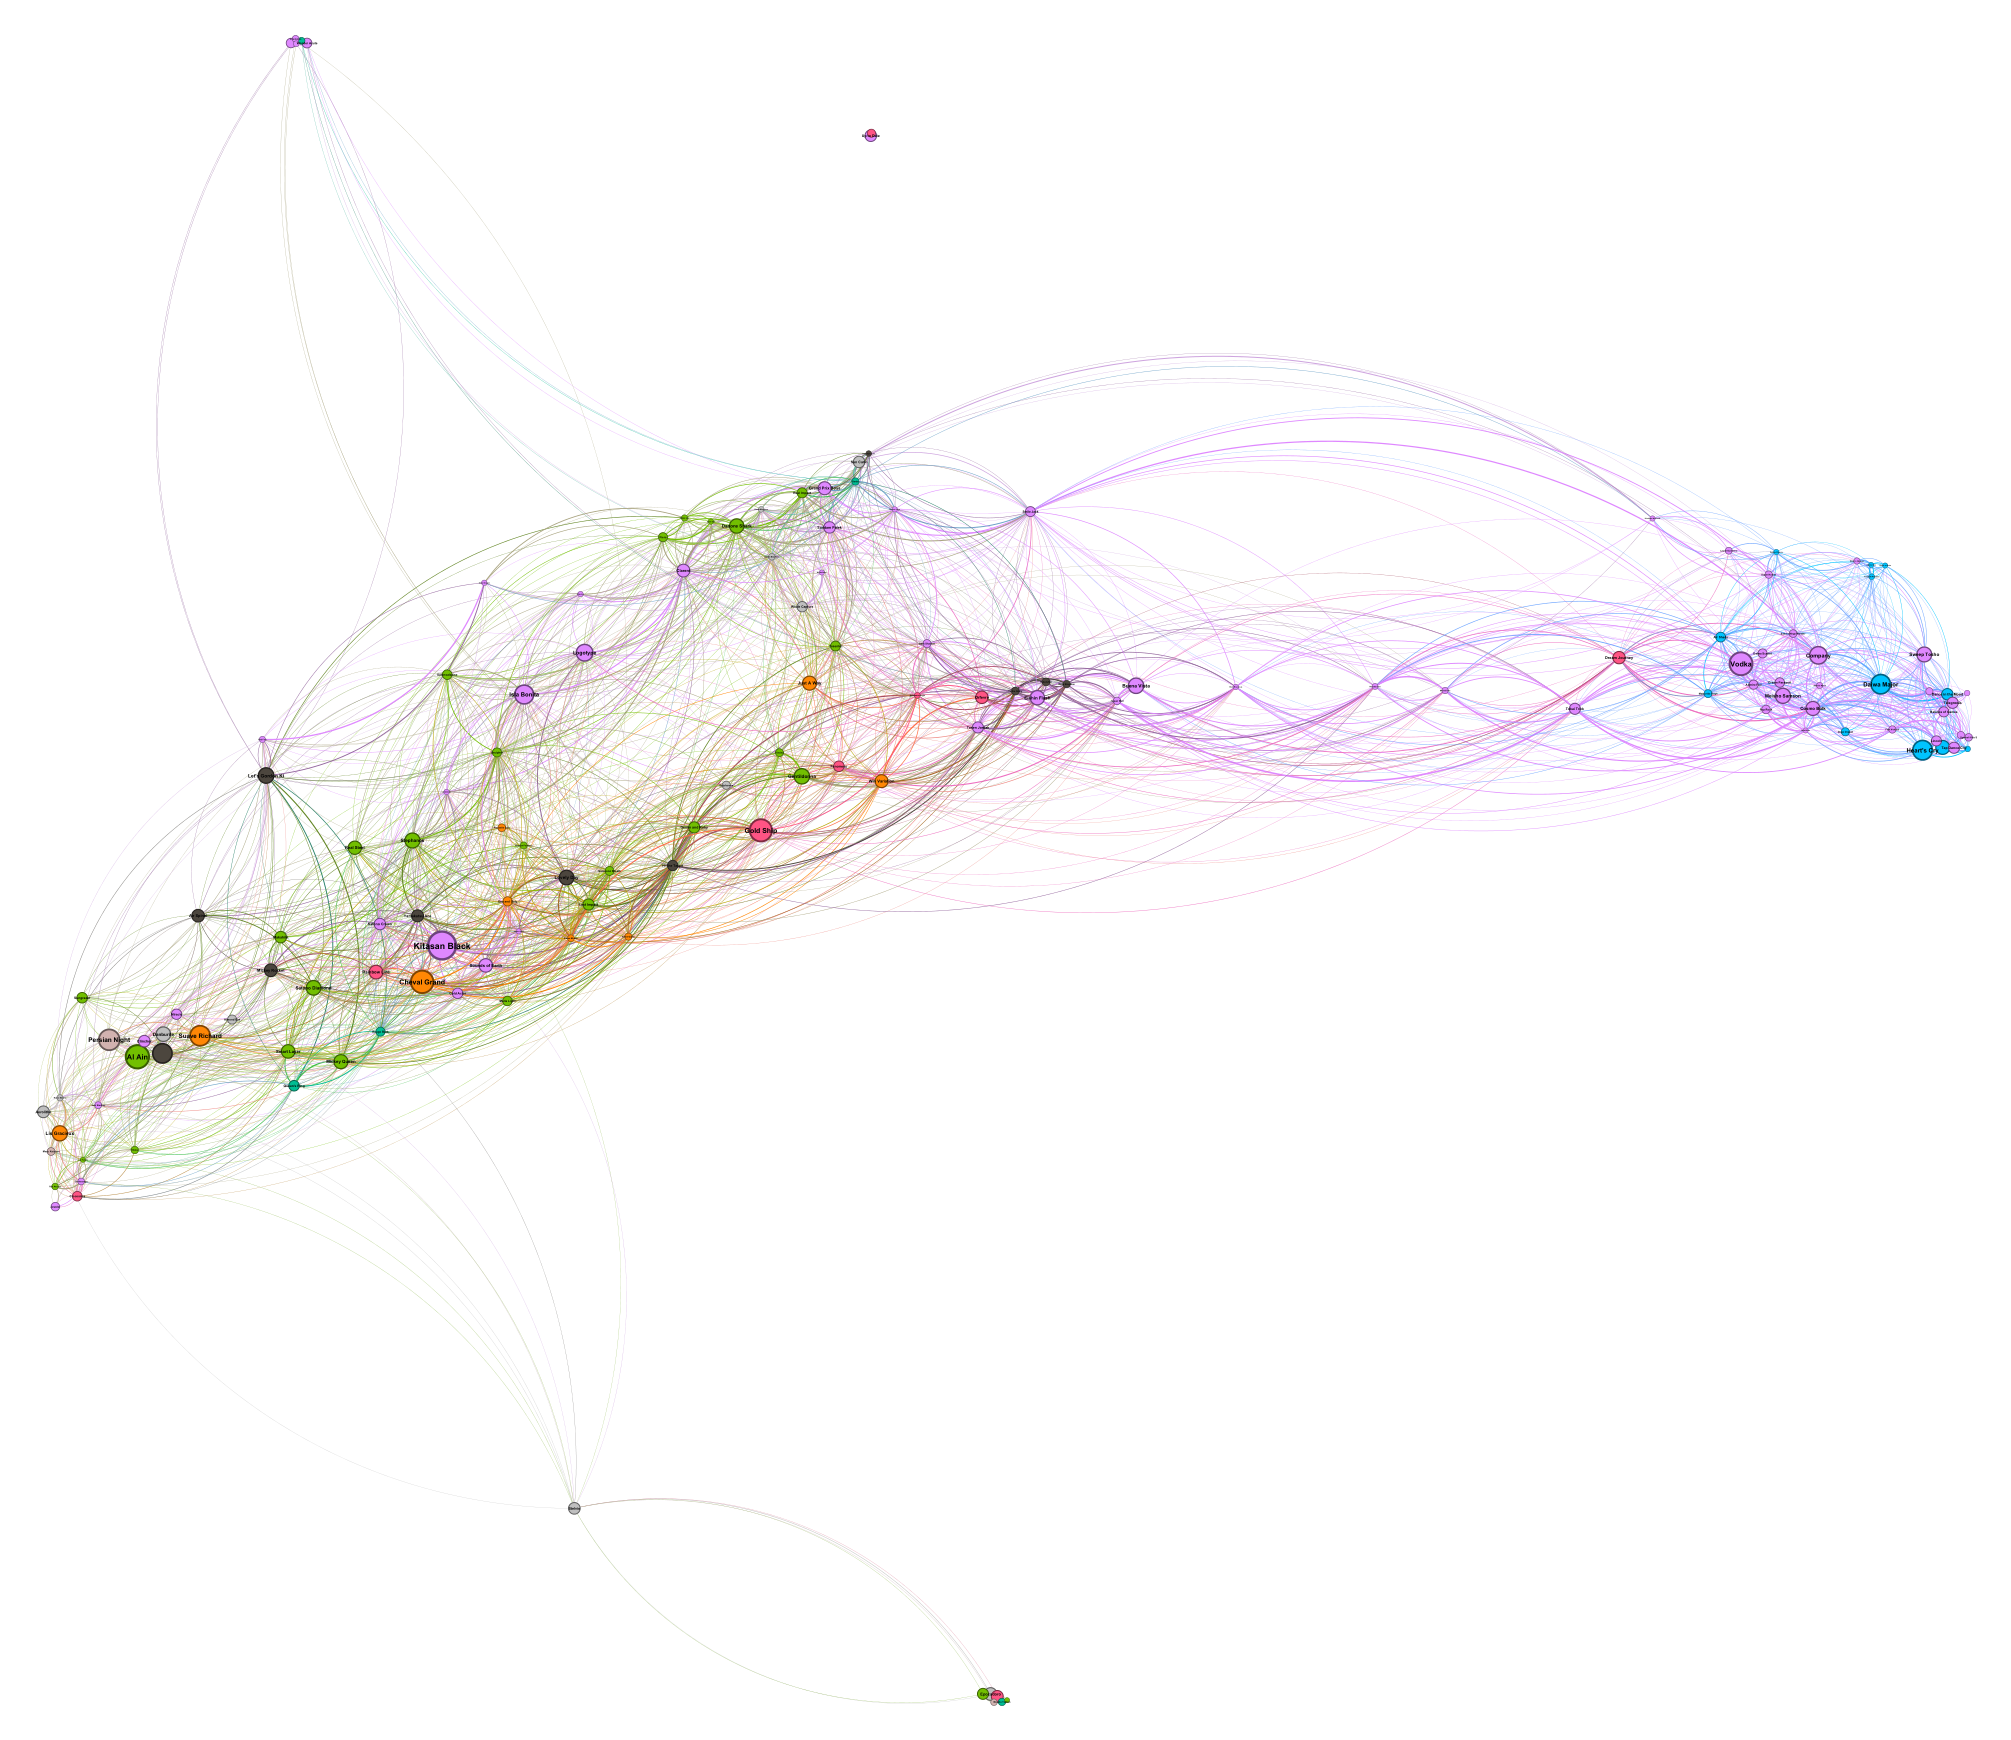
\includegraphics[width=0.82\textwidth]{../assets/gephi_competition_top150.png}\\
{\scriptsize \textbf{Rede de Competição Top 150 PageRank} (2.551 arestas) \& \textbf{Rede Tripartida Jóqueis $\leftrightarrow$ Cavalos $\leftrightarrow$ Treinadores}.}
\end{column}
\begin{column}{0.49\textwidth}
\centering
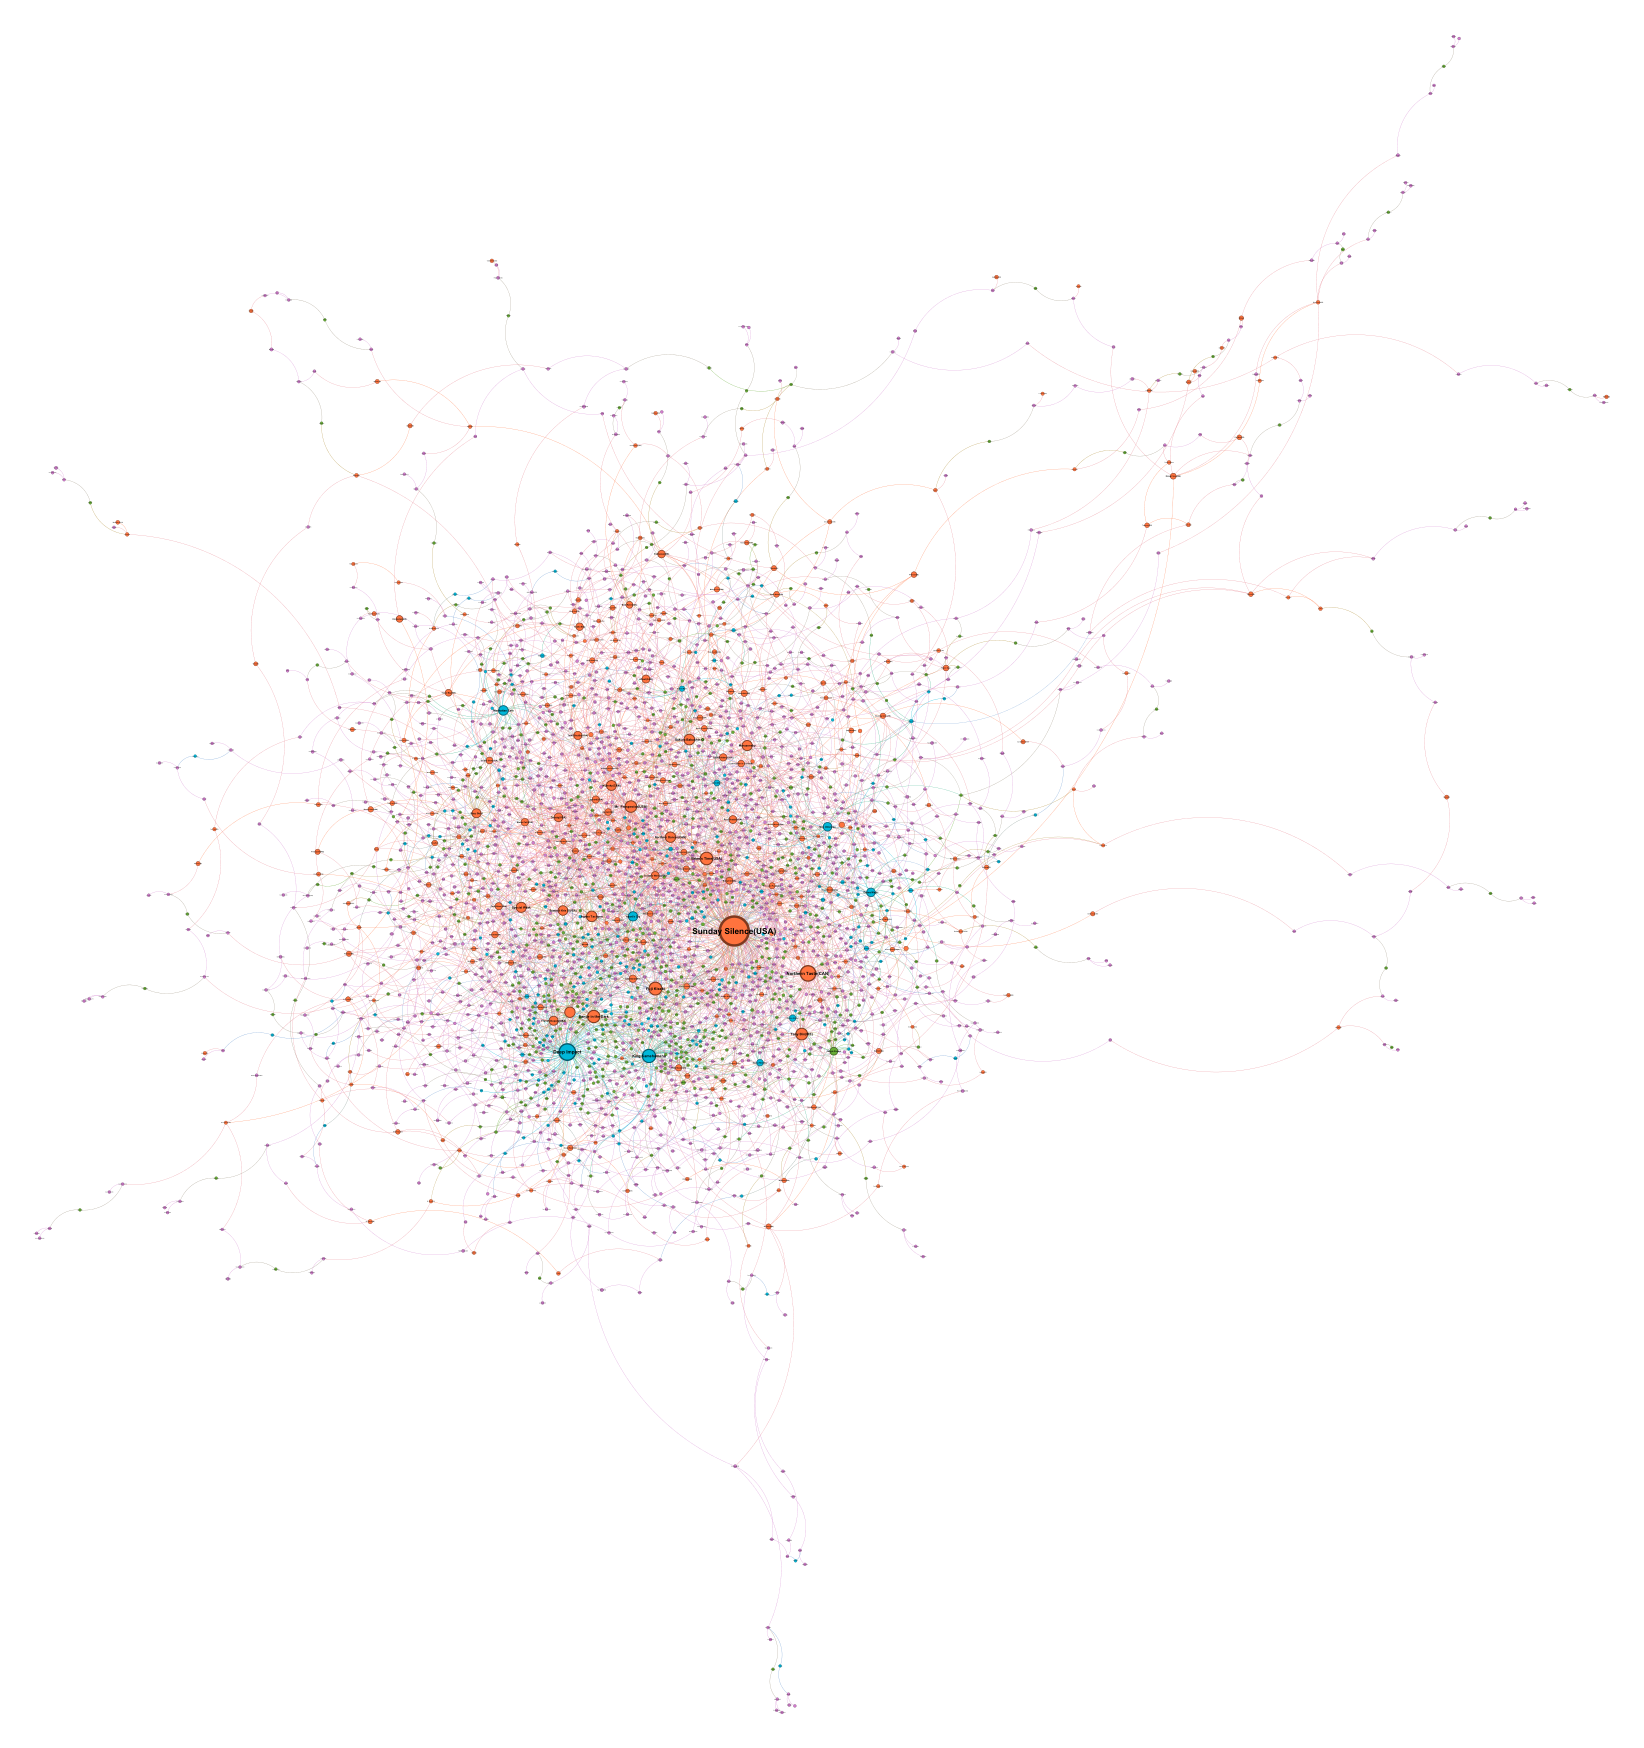
\includegraphics[width=0.82\textwidth]{../assets/gephi_lineage_dag_elite.png}\\
{\scriptsize \textbf{Galáxia Genealógica 5 Gerações (4.475 nós):} Convergência sobre \textit{Northern Dancer} (4.206 cavalos c/ inbreeding, 1.211 vitórias).}
\end{column}
\end{columns}
\end{frame}

% SLIDE 13: SUÍTE INTERATIVA APACHE SUPERSET & GAMIFICAÇÃO TCG ARENA
\begin{frame}{12. Aplicações Web Interativas: Apache Superset Suite \& TCG Arena}
\begin{columns}[T]
\begin{column}{0.48\textwidth}
\begin{block}{🚀 Suíte Interativa Apache Superset / ECharts}
\begin{itemize}
    \footnotesize
    \item \textbf{13 Gráficos Interativos + 6 KPIs} em 3 idiomas (\textbf{PT-BR, EN, JA}) no GitHub Pages.
    \item \textbf{Destaques:} \textit{Drill-Down} clicável no Sunburst dos 10 Hipódromos, Zoom no Quadrante de PageRank e \textbf{Filtro Brush ao Vivo} nas Coordenadas Paralelas!
\end{itemize}
\end{block}
\end{column}
\begin{column}{0.49\textwidth}
\begin{exampleblock}{🃏 Gamificação: JRA \& JBIS TCG Card Arena}
\begin{itemize}
    \footnotesize
    \item \textbf{520 Cards Colecionáveis em 6 Decks de Ranking} (324 Cavalos, 106 Garanhões, 60 Jóqueis e 30 Patriarcas).
    \item \textbf{Raridade Procedural (OVR 76--99):} \texttt{SSR Mythic}, \texttt{DIAMOND Anomaly} (para os Diamantes Injustiçados com 0 vitórias!), \texttt{SILVER Crown}, \texttt{UR} e \texttt{SR}.
    \item \textbf{Dossiê 3D + Árvore Clicável + Modo Duelo (VS)!}
\end{itemize}
\end{exampleblock}
\end{column}
\end{columns}
\vspace{2mm}
\centering
{\footnotesize \textbf{Links Ao Vivo:} \url{https://imarthz.github.io/AEDS2_jra_analysis/docs/superset_interactive_dashboard.html} \\ \url{https://imarthz.github.io/AEDS2_jra_analysis/docs/jra_tcg_arena.html}}
\end{frame}

% SLIDE 14: REPOSITÓRIO CIENTÍFICO E DOI ZENODO
\begin{frame}{13. Repositório Científico, CI/CD e Depósito Oficial no Zenodo}
\begin{block}{Arquitetura de Ciência Aberta e Reprodutibilidade (Item 9)}
\begin{itemize}
    \item \textbf{Repositório GitHub:} \url{https://github.com/ImArthz/AEDS2_jra_analysis}
    \item \textbf{DOI Oficial Emitido no Zenodo (CERN/OpenAIRE):} \textbf{\texttt{10.5281/zenodo.23681764}} (Licença CC-BY-4.0).
    \item \textbf{Estrutura Modular:}
    \begin{itemize}
        \footnotesize
        \item \texttt{data/csv/} (Japonês original) e \texttt{data/csv\_en/} (100\% traduzido para Inglês);
        \item \texttt{data/analysis/} (Rankings PageRank, Inbreeding $F_X$, Clusters K-Means PCA e Random Forest);
        \item \texttt{data/gephi/} (Projetos \texttt{.gephi} e Grafos Vetoriais \texttt{.pdf} com zoom de 1600\%);
        \item \texttt{src/} (12 módulos Python do pipeline de ponta a ponta);
        \item \texttt{.github/workflows/compile\_latex.yml} (CI/CD via GitHub Actions que compila os artigos e slides em PDF via XeLaTeX e publica os Dashboards HTML a cada \textit{push}).
    \end{itemize}
\end{itemize}
\end{block}
\end{frame}

% SLIDE 15: CONCLUSÃO E CONSIDERAÇÕES FINAIS
\begin{frame}{14. Conclusão e Resposta à Pergunta Central}
\begin{exampleblock}{Síntese das 4 Grandes Descobertas Científicas}
\begin{enumerate}
    \item \textbf{A Genética Define ``ONDE'' o Cavalo Vence ($H_1$):} A linhagem paterna de 5 gerações determina com significância extrema ($\chi^2 = 2237,5, p < 10^{-300}$) a aptidão de superfície e distância, dividindo os garanhões em 4 arquétipos (63,4\% de variância no PCA 2D) e revelando dimorfismo biométrico entre Areia ($\approx 496\text{ kg}$) e Grama ($\approx 477\text{ kg}$).
    \item \textbf{A Sinergia Humana e a Forma Atlética Preveem ``QUEM'' Sobe ao Pódio:} No momento da largada, a Random Forest ($\text{ROC-AUC} = 0,7260$ sem vazamento temporal) revelou que a taxa prévia do jóquei (\textbf{29,8\%}) e do cavalo (\textbf{22,7\%}) lideram o poder preditivo.
    \item \textbf{O PageRank Resgata os ``Diamantes Injustiçados'' ($H_2$):} A centralidade em grafos ($r = 0,88$ com pódios) revelou talentos de elite invisíveis à contagem de vitórias, como \textbf{\textit{Sounds of Earth} (\#32 geral entre 8.135 cavalos com 0 vitórias Graded)}.
    \item \textbf{Visualização e Gamificação Democratizam a Ciência dos Dados:} A suíte \textit{Apache Superset / ECharts} e a \textit{TCG Card Arena} (520 cards) tornam modelos matemáticos complexos acessíveis e intuitivos para qualquer público.
\end{enumerate}
\end{exampleblock}
\end{frame}

\end{document}
